\documentclass[a5paper,oneside]{amsart}
\usepackage[scale={.9,.9}]{geometry}
\usepackage{graphicx}
\usepackage{mathrsfs}
\usepackage{amsthm}
\usepackage{amsmath}
\usepackage{amsfonts}
\usepackage{dsfont}
\usepackage[spanish,mexico]{babel}
\usepackage[latin1]{inputenc}
\theoremstyle{plain}
\newtheorem{theorem}{Theorem}
\newtheorem{lemma}{Lemma}
\newtheorem{corollary}{Corollary}
\newtheorem{proposition}{Proposition}
\newtheorem{conjecture}{Conjecture}
\theoremstyle{definition}
\newtheorem{problema}{Problema}
\newtheorem{ejercicio}{Ejercicio}
\newtheorem*{definition}{Definition}
\newtheorem*{remark}{Remark}
\usepackage{listings}
\lstset{
language=R,
basicstyle=%\scriptsize
\ttfamily,
commentstyle=\ttfamily\color{gray},
numbers=none,
numberstyle=\ttfamily\color{gray}\footnotesize,
stepnumber=1,
numbersep=5pt,
backgroundcolor=\color{white},
showspaces=false,
showstringspaces=false,
showtabs=false,
frame=none,
tabsize=4,
captionpos=b,
breaklines=true,
breakatwhitespace=false,
title=\lstname,
escapeinside={},
keywordstyle={},
morekeywords={}
}
\title[Problemas de Procesos I]{Problemas de Procesos Estoc\'asticos I\\ Semestre 2013-II\\ Posgrado en Ciencias Matem\'aticas\\ Universidad Nacional Aut\'onoma de M\'exico}
\author{Ger\'onimo Uribe Bravo}
%\address{}
\usepackage[colorlinks,citecolor=blue,urlcolor=blue]{hyperref}
%\setlength{\textwidth}{17.2cm} % was 18.2
%\setlength{\textheight}{23cm} % was 23
%\setlength{\torgin}{-1cm} % was 0
%\setlength{\oddsidemargin}{-0.6cm}
%\setlength{\evensidemargin}{-0.6cm}

%\setlength{\textwidth}{18.9cm} % was 18.2
%\setlength{\textheight}{26.73cm} % was 23
%\setlength{\topmargin}{1cm} % was 0
%\setlength{\oddsidemargin}{0cm} %
%\setlength{\evensidemargin}{.8cm}
%% Arreglar pues ahora utilizas papel A4.

%Operadores

\DeclareMathOperator{\ivp}{IVP} %
\DeclareMathOperator{\sgn}{sgn} %
\DeclareMathOperator{\md}{mod}
\DeclareMathOperator{\ima}{Im}%
\DeclareMathOperator{\id}{Id} %
\DeclareMathOperator{\homo}{Hom} %
\DeclareMathOperator{\inter}{Int}
\DeclareMathOperator*{\Lim}{lim}
\DeclareMathOperator*{\Limsup}{lim\ sup}
\DeclareMathOperator*{\Liminf}{lim\ inf}
\DeclareMathOperator*{\Min}{m\text{\ii}n}
\DeclareMathOperator{\Aff}{Aff}
\DeclareMathOperator{\Affb}{\overline{\Aff}}
\DeclareMathOperator{\sdfd}{dfd}
\DeclareMathOperator{\scdfd}{dfd}
\DeclareMathOperator{\Beta}{B}
\DeclareMathOperator{\pd}{PD}
\DeclareMathOperator{\supp}{supp}
\DeclareMathOperator{\diam}{diam}
\newcommand{\ind}{\operatornamewithlimits{\perp}}
\DeclareMathOperator{\av}{Abs}
\DeclareMathOperator{\cb}{CB}
\DeclareMathOperator{\cbi}{CBI}
\DeclareMathOperator{\gwi}{GWI}
\DeclareMathOperator{\gw}{GW}
\newcommand{\rtree}{$\re$\nbd tree}
\newcommand{\leb}{\text{Leb}}
%Notaci�n



%Delimitadores
\newcommand{\ceil}[1]{\ensuremath{\lceil #1 \rceil}}
%\renewcommand{\floor}[1]{\ensuremath{\lfloor #1 \rfloor}}

%Formato
\newcommand{\defin}[1]{{\bf #1}}
\newcommand{\mc}[1]{\ensuremath{\mathscr{#1}}}
\newcommand{\bb}[1]{\mathbb{#1}}


%Notation

\newcommand{\card}[1]{\ensuremath{\left| #1 \right|}}
\newcommand{\lccb}{LCCB}
\newcommand{\pss}{S}
\newcommand{\compact}{K}
\newcommand{\psm}{\rho}
\newcommand{\ps}{\paren{\pss,\psm}}
\newcommand{\pse}{x}
\newcommand{\psep}{y}
\newcommand{\psepp}{z}
\newcommand{\saps}{\B_{\pss}}
\newcommand{\bre}{\B_{\re}}
\newcommand{\sko}{D}
\newcommand{\trees}{T}
\newcommand{\C}{C}
\newcommand{\refm}{\mu}
\newcommand{\den}{p}
\newcommand{\psd}[1]{\mc{P}_{#1}}
\newcommand{\s}{\ensuremath{\sigma}}
\newcommand{\bden}{M}
\newcommand{\hh}[1]{{\bf H#1}}
\newcommand{\ball}[2]{\imf{B_{#1}}{#2}}
\newcommand{\mmc}[1]{\imf{\tilde\omega}{#1}}
\newcommand{\rg}[1]{\ensuremath{\imf{\mathbb{G}}{#1}}}




\newcommand{\dfd}{\ensuremath{\stackrel{\sdfd}{=}}}
\newcommand{\deq}{\ensuremath{\stackrel{d}{=}}}

\newcommand{\ley}[2]{\ensuremath{\imf{\mc{L}^{#2}}{#1}}}
\newcommand{\leyc}[3]{\ensuremath{\imf{\mc{L}^{#3}}{#1\left|#2\right.}}}
\newcommand{\cond}[2]{\left.\vphantom{#2}#1\ \right| #2}

\newcommand{\e}{\ensuremath{\mathbf{e}}}
\newcommand{\esf}{\ensuremath{\mc{S}^{\downarrow}}}
%\newcommand{\ps}[1]{\mathscr{P}\paren{#1}}
\newcommand{\fun}[3]{\ensuremath{#1:#2\to #3}}
\newcommand{\fund}[3]{\ensuremath{#1:#2\mapsto #3}}
\newcommand{\set}[1]{\ensuremath{\left\{ #1\right\} }}
\newcommand{\sets}[1]{\ensuremath{{\mathbf #1}}}
\newcommand{\paren}[1]{\ensuremath{\left( #1\right) }}
\newcommand{\bra}[1]{\ensuremath{\left[ #1\right] }}
\newcommand{\seq}[1]{\ensuremath{ #1 _1,\ldots ,#1 _n }}
\newcommand{\sm}[3]{\left[ #1\right]_{#2}^{#3}}
\newcommand{\cde}{\Rightarrow}
\newcommand{\cdfd}{\ensuremath{\stackrel{\scdfd}{\cde}}}
\newcommand{\convo}[2]{\ensuremath{#2^{\!* #1}}}

\newcommand{\tl}[1]{\ensuremath{\hat{#1}}}

\newcommand{\matt}[3]{#1_{#2\, #3}}
\newcommand{\sip}{\bb{P}}
\newcommand{\jump}[2]{\ensuremath{\Delta #1_{#2}}}
\newcommand{\cadlag}{c\`adl\`ag}
\newcommand{\se}{\ensuremath{\bb{E}}}
\newcommand{\ssa}{\ensuremath{\mathscr{F}}}
\newcommand{\si}{{\ensuremath{\bf{1}}}}
\newcommand{\sbr}{\ensuremath{\mc{B}_{\re}}}
%\newcommand{\siind}{\ensuremath{\perp}}
\newcommand{\sigam}{\ensuremath{\Gamma}}
\newcommand{\smc}{\ensuremath{m}}
\newcommand{\sfleche}{S^{\downarrow}_f}

\newcommand{\gafun}[1]{\sigam \paren{#1}}
\newcommand{\poi}[1]{\ensuremath{\mc{P}\!_{#1}}}
\newcommand{\ber}[1]{\ensuremath{\mc{B}\!_{#1}}}
\newcommand{\fcpoi}[1]{\ensuremath{\hat{\mc{P}}\!_{#1}}}
%\newcommand{\ind}{\siind}
\newcommand{\condind}[3]{\ensuremath{#1\ind_{#3}#2}}
\newcommand{\sig}[1]{$\sigma$-\nobreakdash #1}
\newcommand{\sa}{\ensuremath{\sigma}\nbd field}
\newcommand{\realtree}{\ensuremath{\re}\nbd tree}
\newcommand{\eps}{\ensuremath{ \varepsilon}}
\newcommand{\na}{\ensuremath{\mathbb{N}}}
\newcommand{\en}{\ensuremath{\mathbb{Z}_+}}
\newcommand{\eti}{\ensuremath{\mc{U}}}
\newcommand{\etic}{\ensuremath{\mathbb{U}}}
\newcommand{\z}{\ensuremath{\mathbb{Z}}}
\newcommand{\re}{\ensuremath{\mathbb{R}}}
\newcommand{\ra}{\ensuremath{\mathbb{Q}}}
\newcommand{\com}{\ensuremath{\mathbb{C}}}
\newcommand{\con}[1]{\ensuremath{\overline{#1}}}
\newcommand{\proba}[1]{\ensuremath{\sip\! \left( #1 \right)}}
\newcommand{\probas}[2]{\ensuremath{#1\! \left( #2 \right)}}
\newcommand{\probac}[2]{\ensuremath{\sip\! \left( #1 \, | #2 \right)}}
\newcommand{\esp}[1]{\ensuremath{\se\! \left( #1 \right)}}
%\newcommand{\espc}[2]{\ensuremath{\se\! \left( #1 | #2 \right)}}
\newcommand{\espc}[2]{\ensuremath{\imf{\se}{\cond{#1}{#2}}}}
\newcommand{\var}[1]{\ensuremath{\text{Var}\! \left( #1 \right)}}
\newcommand{\cov}[1]{\ensuremath{Cov\! \left( #1 \right)}}
\newcommand{\abs}[1]{\hspace{.25mm}\left|#1\right|\hspace{.25mm}}
\newcommand{\ila}[2]{\ensuremath{\int #1\, d#2}}
\newcommand{\ilas}[3]{\ensuremath{\int_{#1} #2\, d#3}}
\newcommand{\il}[3]{\ensuremath{\int #1\, \imf{#2}{d#3}}}
\newcommand{\is}[4]{\ensuremath{\int_{#1} #2\, \imf{#3}{d#4}}}
\newcommand{\lp}[2]{\ensuremath{\mc{L}_#1\!\paren{#2} }}
\newcommand{\lpc}[4]{\ensuremath{\mc{L}_#1\!\paren{ #2 , #3 , #4 }}}
\newcommand{\ip}[1]{\ensuremath{\int #1\, d\sip }}
\newcommand{\ips}[2]{\ensuremath{\int_{#1} #2\, d\sip}}
\newcommand{\F}{\ssa}
\newcommand{\uF}{\ssa^u}
\newcommand{\G}{\ensuremath{\mc{G}}}
\newcommand{\h}{\ensuremath{\mc{H}}}
\newcommand{\B}{\ensuremath{\mc{B}}}
\newcommand{\f}[1]{\ssa_{#1}}
\newcommand{\fx}[2]{\ssa_{#1}^{#2}}
\newcommand{\indi}[1]{\si_{#1}}
\newcommand{\imi}[2]{#2^{-1}\!\paren{#1}}
\newcommand{\ooo}{\ensuremath{ \omega  } }
\newcommand{\oo}{\ensuremath{ \Omega  } }
\newcommand{\p}{\ensuremath{ \sip  } }
\newcommand{\q}{\ensuremath{ \bb{Q}  } }
\newcommand{\ofp}{\ensuremath{ \paren{ \Omega ,\F ,\p } } }
\newcommand{\med}[2]{\ensuremath{\paren{#1}{#2}}-medible}
\newcommand{\vat}{\ensuremath{\fun{X}{\oo}{\re}}\ }
\newcommand{\pix}[1]{\ensuremath{\sip}_{\! #1}}
\newcommand{\px}[2]{\ensuremath{\sip_{\! #1}\!\paren{#2}}}
\newcommand{\pxc}[3]{\ensuremath{\sip_{\! #1}\!\left( #2 | #3 \right)}  }
\newcommand{\br}{\sbr}
\newcommand{\sag}[1]{\sigma\!\paren{#1}}
\newcommand{\cs}[1]{\ensuremath{#1}-p.s.}
\newcommand{\ore}{ \ensuremath{\overline{\re}}}
\newcommand{\fungen}[1]{\ensuremath{\varphi_{#1}}}%Comando para la notaciÛn de funciÛn generadora.
\newcommand{\cbin}[2]{\ensuremath{\paren{\begin{array}{c}#1\\#2\end{array}}}}
\newcommand{\fa}[2]{\ensuremath{{#1}^{\paren{#2}}}}
\newcommand{\dnor}[2]{\ensuremath{N(#1,#2)}}
\newcommand{\mb}{movimiento browniano}
\newcommand{\moc}[3]{\smc^{#3}(#1,#2)}
\newcommand{\clo}[1]{\ensuremath{\overline{#1}}}
\newcommand{\inte}[1]{\ensuremath{\inter #1}}
\newcommand{\fro}[1]{\ensuremath{\partial\paren{ #1}}}
\newcommand{\cd}[2]{\ensuremath{#1\stackrel{\mc{D}}{\to}#2}}
\newcommand{\pr}[3]{\ensuremath{#1_{#2}\!\paren{#3}}}
\newcommand{\oi}[1]{\ensuremath{\mc{O}\paren{#1}}}
\newcommand{\mw}{\ensuremath{\mathbb{P}}}
\newcommand{\me}{\ensuremath{\pi}}


\newcommand{\nbd}{\nobreakdash -}
\newcommand{\ii}{\'{\i}}
\newcommand{\n}{\~n}
\newcommand{\imf}[2]{\ensuremath{#1\!\paren{#2}}}
\newcommand{\floor}[1]{\ensuremath{\lfloor #1\rfloor}}
\newcommand{\proint}[2]{\ensuremath{\langle #1,#2\rangle}}
\newcommand{\vp}{\ensuremath{\varphi}}
\newcommand{\noru}[1]{\ensuremath{\|#1\|}}
\newcommand{\gen}[1]{\ensuremath{|#1 |}}
\newcommand{\vc}[1]{\ensuremath{\langle #1\rangle}}
\newcommand{\pc}[2]{\ensuremath{\langle#1,#2\rangle}}
\newcommand{\vcd}[1]{\ensuremath{\left[#1\right]}}

\newcommand{\sml}{\ensuremath{\nu}}
\newcommand{\ml}[1]{\ensuremath{\imf{\sml}{#1}}}
\newcommand{\va}[2]{\ensuremath{\imf{V_{#1}}{#2}}}
\newcommand{\clase}[1]{\ensuremath{\mc{C}^{#1}}}
\newcommand{\marte}[2]{\ensuremath{\imf{\mc{E}^{#2}}{#1}}}

\newcommand{\dencero}[1]{\ensuremath{\left. \frac{\partial }{\partial #1}\right|_{#1=0} }}
%\newcommand{\premin}[1]{\ensuremath{\stackrel{\leftarrow}{#1}}}
%\newcommand{\postmin}[1]{\ensuremath{\stackrel{\rightarrow}{#1}}}
\newcommand{\premin}[1]{\ensuremath{{#1}^{\leftarrow}}}
\newcommand{\postmin}[1]{\ensuremath{{#1}^{\rightarrow}}}



%Ambientes (Environments)

\newenvironment{esn}{\begin{displaymath}}{\end{displaymath}}
\newenvironment{ecn}{\begin{equation}}{\end{equation}}
\newenvironment{listeo}{\begin{list}{\alph{enumi})}{\usecounter{enumi}}}{\end{list}}
\newenvironment{numerai}{\begin{list}{\roman{enumi})}{\usecounter{enumi}}}{\end{list}}
%\usepackage[colorlinks,citecolor=blue,urlcolor=blue]{hyperref}
\begin{document}
\maketitle

\newcommand{\nats}{\mathds{N}}
\newcommand{\reals}{\mathds{R}}
\newcommand{\entpos}{\mathds{Z}_{+}}
\newcommand{\prob}{\mathds{P}}
\newcommand{\mean}{\mathds{E}}
\newcommand{\mat}[1]{{\bm #1}}
\newcommand{\nota}[1]{\hspace{5 mm}\mbox{#1}}
\newcommand{\tres}{\hspace{3 mm}}
\newcommand{\cinco}{\hspace{5 mm}}
\newcommand{\uno}{\hspace{1 mm}}
\newcommand{\ent}{\Rightarrow}
\newcommand{\sii}{\Leftrightarrow}
\newcommand{\borr}{\mathds{B}_{\mathds{R}}}
\begin{problema}
Sean $\paren{X_n}_{n\in\na}$ un proceso estoc\'astico con valores reales y $A\subset\re$ un boreliano. Pruebe que si\begin{esn}
T_0=0\quad\text{y}\quad T_{n+1}=\min\set{k>T_n: X_k\in A}
\end{esn}entonces $T_n$ es un tiempo de paro para toda $n$ y $T_n\to \infty$ puntualmente conforme $n\to\infty$. 

\defin{Categor\'ias: } Tiempos de paro
\end{problema}


\begin{proof}
Sean $\F_0 = \{\emptyset , \Omega\}$ y $\F_n = \sigma (X_1 , X_2 , \dots , X_n )$. Se demostrar\'a por inducci\'on. Sea $B\in\borr$.

$\ent$
\[T_0^{-1} (B) = \left\{\begin{array}{ccc}
\Omega & \mbox{ si } & 0\in B \\ 
\emptyset & \mbox{ si } & 0\notin B
\end{array} \right.\] 
Por lo tanto, $T_0$ es $\F_0$-medible y en particular $\{T_0=j \}\in \F_0\subset\F_j$ para todo $j\in\nats$, de manera que $T_0$ es un tiempo de paro. 

Ahora supongamos que $T_n$ es tiempo de paro, es decir, $\{T_n=j\}\in\F_j$ para todo $j\in\nats$. Consideremos el evento $\{T_{n+1} = k\}$ y notemos que
\[\{T_{n+1}= k\} = \left(\cup_{j=1}^{k-1} \{T_n=j\}\cap\left(\cap_{i=j+1}^{k-1} \{X_i\notin A\}\right)\right)\cap\{X_{k}\in A\}.\]

Por hip\'otesis inductiva, cada $\{T_n=j\}\in \F_j\subset\F_k$. Tambi\'en $\{X_i\notin A\}\in \F_i\subset\F_k$ y por \'ultimo $\{X_{k}\in A\}\in\F_k$. $F_k$ es cerrado bajo intersecciones y uniones, por lo tanto $\{T_{n+1}= k\}\in\F_k$. Lo anterior es v\'alido para cualquier $k\in\nats$, por lo tanto $T_{n+1}$ es un tiempo de paro.

Para demostrar que $T_n \rightarrow \infty$ cuando $n\rightarrow\infty$, basta demostrar que $T_n\ge n$, de nuevo, por inducci\'on.

Por definici\'on, $T_0\ge 0$. Ahora supongamos que $T_n\ge n$. Entonces pueden suceder 2 cosas.
\[\{k> T_n : X_k \in A\} = \emptyset \ent T_{n+1} = \infty \ge n+1.\]
En caso contrario, $T_{n+1}=\min\{k> T_n : X_k \in A\}>T_n\ge n$. Por lo tanto, $T_{n+1}\ge n+1$.

En cualquier caso, la desigualdad se cumple y si hacemos $n\rightarrow\infty$, tenemos que $T_n \rightarrow \infty$.
\end{proof}

\begin{problema}[Lo que siempre tiene una posibilidad razonable de suceder lo har\'a; (casi seguramente)-- y pronto]
\emph{Tomado de \cite[E10.5, p.223]{MR1155402}}

Suponga que \(T\) es un tiempo de paro tal que para alg\'un \(N\in\na\) y \(\varepsilon>0\) se tiene que para toda \(n\in\na\):
 $$
 \p (T\leq N+ n|\F_n)>\varepsilon \text{ casi seguramente}
 $$
Al verificar la desomposici\'on
 $$
\p (T>kN)= \p (T>kN,T>(k-1)N),
 $$pruebe por inducci\'on que para cada \(k=1,2,\ldots\):
 $$
\p (T>kN)\leq \paren{1-\eps}^k. 
 $$Pruebe que \( \esp{T}<\infty \).
 
 \defin{Categor\'ias:} Tiempos de paro.
\end{problema}
\begin{proof}
Sea $k\in\nats$. Notemos que $\{T> k N\}\subset\{T > (k-1)N\}$ y por lo tanto, $\{T > (k-1)N, T> k N\} = \{T> k N\}$. Esto implica que $\p (T> k N) = \p (T > (k-1)N, T> k N)$.

Queda por demostrar que $\p ( T > kN)\le (1-\eps )^k$, lo cual se har\'a por inducci\'on. 

Consideremos el caso $k=1$. Entonces,
\begin{align*}
\p (T>N) & = \mean (\p (T>N + 0 | \F_0 ) )\\
& = \mean (1-\eps) = 1- \eps, 
\end{align*}
desmostrando que la desigualdad es v\'alida en este caso.

Ahora supongamos que la desigualdad es v\'alida para $k-1\in\nats$, es decir, que $\p ( T > (k-1)N)\le (1-\eps )^{k-1}$. Entonces,
\begin{align*}
\p (T > kN) & = \p (T > (k-1)N, T> k N)\\
& = \mean (\mean (\mathds{1}_{T>(k-1)N}\mathds{1}_{T>kN} |\F_{(k-1)N} ))\\
& = \mean (\mathds{1}_{T>(k-1)N} \mean (\mathds{1}_{T>kN} |\F_{(k-1)N} ))\\
& \nota{(Por que $\{T>(k-1)N\} = \{T\le (k-1)N\}^{c}\in \F_{(k-1)N}$)}\\
& = \mean (\mathds{1}_{T>(k-1)N} \p(T>kN |\F_{(k-1)N} ))\\
& = \mean (\mathds{1}_{T>(k-1)N} \p(T>N + (k-1)N |\F_{(k-1)N} ))\\
& \le \mean (\mathds{1}_{T>(k-1)N} (1-\eps ))\nota{(Por monoton\'ia)}\\
& = \p (T>(k-1)N )(1-\eps ) \le (1-\eps )^{k-1} (1-\eps )\nota{(Por hip. ind.)}\\
& = (1-\eps )^k,\\
\end{align*}
finalizando la prueba inductiva.

Ahora intentemos acotar $\mean (T)$. Notemos que para todo $k\in\entpos$, $\p (T>kN)\ge \p (T>kN + 1) \ge \p (T>kN + (N-1))$.

\begin{align*}
\mean (T) & = \sum_{j=1}^\infty \p (T\ge j) = \sum_{j=0}^\infty \p (T > j)\\
& \le \sum_{j=0}^{N-1} + \sum_{j=N}^\infty \p (T > j)\\
& \le N-1 + \sum_{k=1}^\infty N \p (T > kN)\\
& = N-1 + N \sum_{k=1}^\infty (1-\eps )^k\\
& = N-1 + N(1-\eps )/\eps < \infty .
\end{align*}
\end{proof}
\begin{problema}
\emph{Tomado de Mathematical Tripos, Part III, Paper 33, 2012, \url{http://www.maths.cam.ac.uk/postgrad/mathiii/pastpapers/}}


Sean $\paren{X_i,i\in\na}$ variables aleatorias independientes con $\proba{X_i=\pm 1}=1/2$. Sean $S_0=0$ y $S_n=\sum_{i=1}^n X_i$. 
\begin{enumerate}
\item Sea $T_1=\min\set{n\geq 0:S_n=1}$. Explique por qu\'e $T_1$ es un tiempo de paro y calcule su esperanza.
\begin{proof}
Sea $F_0=\{\emptyset,\Omega\}$ y $\F_n=\sigma (X_1,\dots ,X_n )$. Consideremos
\[\{T_1=n\} = \left(\cap_{j=0}^{n-1} \{S_j \neq 1\}\right) \cap \{S_n = 1\}.\]
Es claro que $S_0$, una funci\'on constante, es $\F_0$-medible. Como $S_j = f(X_1,\dots , X_j)$, entonces $S_j$ es $\F_j$-medible para todo $j\in\nats$. As\'i pues, cada $\{S_j \neq 1\}\in \F_j\subset\F_n$ y $\{S_n = 1\} \in \F_n$. Como $\F_n$ es cerrada bajo intersecciones, entonces $\{T_1=n\}\in \F_n$.

Para calcular $\mean (T_1)$, definamos $T_x=\inf \{n\ge : S_n = x\}$. Para todo $a,b\in \nats$, el resultado del Problema de la Ruina (visto en clase), dice que
\[\mean (T_{-a}\wedge T_{b}) = ab.\]

Notemos que $T_{-(a+1)} > T_{-a}$ (antes de llegar al nivel $-(a+1)$, el proceso $S$ debi\'o haber pasado por el nivel $-a$), es decir $\{T_{-n}\}_{n\in\nats}$ es una sucesi\'on de v.a. estrictamente creciente que toma valores en $\nats$. Por lo tanto, $\lim_{n\rightarrow\infty} T_{-n} = \infty$. As\'i pues, $\lim_{n\rightarrow\infty} T_{-n}\wedge T_1 = T_1$. Ademas, $\{T_{-n}\wedge T_1\}_{n\in\nats}$ es una sucesi\'on no decreciente de v.a. y entonces, por TCM,
\[\mean (T_1) = \lim_{n\rightarrow\infty} \mean (T_{-n}\wedge T_1 ) = \lim_{n\rightarrow\infty} n\cdot 1 = \infty .\]

Para demostrar que $\p (T_1 < \infty ) = 0$, utilizaremos el resultado obtenido en el Problema de la Ruina,
\[\p (T_{b} < T_{-a}) = a/(a+b),\]
de manera que por continuidad de la funci\'on de probabilidad,
\[\p (T_{1} < \infty ) = \lim_{n\rightarrow\infty} \p (T_{1} < T_{-n}) = \lim_{n\rightarrow\infty} n/(n+1) = 1, \]
terminando con la demostraci\'on.
\end{proof}
\item Mediante el inciso anterior, construya una martingala que converge casi seguramente pero no lo hace en $L_1$.
\begin{proof}
Si $T_1$ es un tiempo de paro, entonces $T_1\wedge n$ tambien ser\'a un tiempo de paro, para toda $n\in\nats$. Definamos
\[M_n:= S_{T_1\wedge n}.\]
Sea $A\in\borr$. Entonces,
\[\{M_n \in A\} = \left(\cup_{j=0}^n \{S_j\in A, T = j\}\right)\cup \{S_n\in A, T > n\}.\]
Cada $\{S_j\in A\}\in\F_j\subset\F_n$ y $\{T_1>n\}=\{T_1\le n\}^{c}\in\F_n.$ Como $\F_n$ es cerrado bajo intersecciones y uniones, $\{M_n\in A\}\in\F_n$, es decir, $M_n$ es $\F_n$-medible. 

Notemos que $|M_n|\le \sum _{i=0}^n |S_i|$, y como cada $S_i$ es una suma de funciones en $L_1$, $S_i\in L_1$ y por lo tanto $M_n \in \L_1$.

Por \'ultimo, veamos que
\begin{align*}
\mean (M_{n+1} | \F_n) & = \mean (S_{T_1\wedge n} | \F_n) = \mean \left(\sum_{i=1}^{n+1} X_i\mathds{1}_{i\le T} | \F_n\right)\\
& = \mean \left(\sum_{i=1}^{n+1} X_i\mathds{1}_{i-1 < T} | \F_n\right)\\
& = \sum_{i=1}^{n} X_i\mathds{1}_{i-1 < T} + \mean (X_{n+1}\mathds{1}_{n<T}|\F_n)\\
& \nota{(Por linealidad de la esp. cond. y $\F_n$ medibilidad de $X_i$ y $\mathds{1}_{i-1 < T}$)}\\
& = \sum_{i=1}^{n} X_i\mathds{1}_{i-1 < T} + \mathds{1}_{n<T}\mean (X_{n+1})\\
& \nota{(Por $\F_n$-medibilidad de $\mathds{1}_{n<T}$ e independencia de $X_{n+1}$ con $\F_n$)}\\
& = \sum_{i=1}^{n} X_i\mathds{1}_{i-1 < T} + \mathds{1}_{n<T}\cdot 0\\
& = \sum_{i=1}^{n} X_i\mathds{1}_{i-1 < T} = S_{T_1\wedge n} = M_n,
\end{align*}
de manera que $M_n$ es una $\F_n$-martingala. 

Notemos que $T_1\wedge n$ es un tiempo de paro acotado, entonces aplicando el Teorema de Muestreo Opcional, tenemos que para todo $n\in\nats$,
\[\mean (M_n) = \mean (S_{T_1\wedge n}) = \mean (S_{0}) = 0.\]

Por otro lado, consideremos $N_n:= -M_n +1$. Claramente $N_n$ es $\F_n$-medible debido a que se trata de una funci\'on continua de $M_n$ y $\mean (|N_n|) \le \mean(|M_n|) + 1 < \infty$, por lo tanto, $N_n \in L_1$. Adem\'as, 
\[\mean (N_{n+1} | \F_n) = -\mean (M_{n+1}) + 1 = -M_n + 1 = N_n,\]
por lo tanto, $N_n$ es una $\F_n$-martingala, que adem\'as ser\'a no negativa. Entonces, por el Teorema de Convergencia de Martingalas (TCMgls),
existe $N_\infty \in L_1$ tal que $N_n\rightarrow N_\infty$ c.s., lo cual implica que existe $M_\infty \in L_1$ tal que $M_n\rightarrow M_\infty$ c.s.. Recordemos que $\{T_1<\infty\}$ casi seguramente, de manera que de hecho $S_{T_1}=M_\infty$ c.s..

Para demostrar que $M_n \rightarrow S_{T_1}$ en $L_1$ no es v\'alida, basta ver que $\mean (S_{T_1}) = 1$ y $\mean (M_n) = 0$ para todo $n\in\nats$, de manera que la convergencia en $L_1$ es imposible.
\end{proof}
\item Sea $M_n$ la martingala obtenida al detener a $-S$ en $T_1$. Utilice la soluci\'on al Problema de la Ruina para probar que $\proba{\max_n M_n\geq M}=1/M$ para todo $M\geq 1$. Concluya que \(\esp{\max_m M_m}=\infty\) y que por lo tanto \(\esp{\max_{m\leq n}M_n}\to\infty\) conforme \(n\to\infty\). Finalmente, deduzca que no puede haber una desigualdad tipo Doob cuando \(p=1\).
\begin{proof}
Consideremos mejor la martingala $N_n := -M_n + 1$, donde $N_n$ y $M_n$ son como en el inciso anterior, la cual es positiva y por lo tanto, $N_n^{+} = N_n$ para todo $n\in\nats$. 
Notemmos que
\begin{align*}
\{\max_n N_n \ge M\} & = \{\max_n (-M_n) \ge M - 1\} \\
& = \cup_{i=0}^\infty \left(\{M_i=-(M-1)\} \cap_{j=0}^{i-1} \{M_j\neq -1\}\right)\\
& = \{T_{-(M-1)} < T_1\}
\end{align*}
Utilizando el resultado correspondiente del Problema de la Ruina, tenemos que
\[\p (\max_n N_n \ge M) = \p (T_{-(M-1)} < T_1) = \frac{1}{(M-1) + 1} = \frac{1}{M}.\]
\[\ent \mean (\max_n N_n) = \sum_{i=1}^\infty \p (\max_n N_n \ge i) = \sum_{i=1}^\infty\frac{1}{i} = \infty .\]

Por otra parte, notemos que $\max_{m\le n} N_m$ es una funci\'on creciente respecto a $n$ y por TCM,
\[\lim_{n\rightarrow \infty}\mean(\max_{m\le n} N_m) = \mean (\max_n N_n) = \infty .\]
Por el inciso anterior (consecuencia del Teorema de Muestreo Opcional de Doob), $\mean (N_m) = 1$ para todo $m\in\nats$ y por lo tanto no existe $k\in\reals$ tal que 
\begin{align*}
\mean & (\max_{m\le n} N_m)\le k\mean (N_n) = k\\
& \nota{(Debido a que $\mean (\max_{m\le n} N_m)$ tiende a $\infty$ cuando $n\rightarrow\infty$)}
\end{align*}
que corresponder\'ia a la Desigualdad $L_p$ de Doob para el caso $p=1$ (que justamente vimos, no se cumple).
\end{proof}
\item Sea $T=\min\set{n\geq 2:S_n=S_{n-2}+2}$ y $U=T-2$. ?`Son $T$ y $U$ tiempos de paro? Justifique su respuesta.
\begin{proof}
Sea $k\in\nats$. Es claro que si $k=0$ o $k=1$, $\{T\le k\}=\emptyset$, el cual es elemento de cualquier $\sigma$-\'algebra. Consideremos $k\ge 2$. Entonces
\begin{align*}
\{T\le k\} & = \cup_{i=2}^k \{S_i = S_{i-2} + 2\}\\
& = \cup_{i=2}^k \{X_{i-1} = 1, X_i = 1\},
\end{align*}
donde los conjuntos $\{X_{i-1} = 1, X_i = 1\}\in\F_i\subset\F_k$, de manera que $\{T\le k\}\in\F_k$ y por lo tanto, $T$ es un tiempo de paro.

Por otro lado, de nuevo consideremos un $k\in\nats$, $k\ge 2$,
\begin{align*}
\{U\le k\} & = \{T\le k + 2\} = \cup_{i=2}^{k+2} \{S_i = S_{i-2} + 2\}\\
& = \cup_{i=2}^{k+2} \{X_{i-1} = 1, X_i = 1\}\\
& = \left(\cup_{i=2}^{k} \{X_{i-1} = 1, X_i = 1\}\right)\cup\{X_{k} = 1, X_{k+1} = 1\}\cup\{X_{k+1} = 1, X_{k+2} = 1\}.
\end{align*}
Pero los eventos $\{X_{k+1} = 1\}$ y $\{ X_{k+2} = 1\}$ no son (necesariamente) $\F_k$-medibles, y entonces $\{U\le k\}\notin\F_k$. Por lo tanto, $U$ no es un tiempo de paro.
\end{proof}
\item Para la variable $T$ que hemos definido, calcule $\esp{T}$. 
\begin{proof}
Para calcular $\mean (T)$, antes decribiremos un juego que despues demostraremos corresponde a una martingala. Supongase que se tiene una sucesi\'on de v.a. i. i. d.$\{X\}$ que valen -1 con probabilidad 1/2 y 1 con probabilidad 1/2. Notemos que si hacemos $Y_n=(X_n+1)/2$ para toda $n\in\nats$, entonces $\{Y\}$ son v.a.i.i.d. $Ber(1/2)$. Un casino basa un juego en este proceso; a cada tiempo $i$, llega un jugador (distinto) con un peso y lo apuesta a que $X_i=1$. Si gana, recibe 2 pesos y si pierde, no se le regresa su d\'olar. En el caso en el gane, vuelve a apostar los 2 pesos que gano a que $X_{i+1}=1$, de manera que si vuelve a atinarle, el casino le dar\'a 4 pesos (momento en el que suceder\'a el tiempo de paro $T$ y se detendr\'a el juego); si pierde, no se le regresar\'an los 2 pesos. Este proceso representa un juego justo e intuitivamente ser\'a una martingala. Para demostrarlo formalmente, sea entonces
\[M_n^i = \mbox{La ganancia del jugador $i$-\'esimo al tiempo $n$.}\]
Bajo la explicaci\'on anterior (y suponiendo que el jugador no para de apostar lo que recibe)
\[M_n^i = (M_{n-1}^i + 1)2\mathds{1}_{X_n=1} - 1,\mbox{ definida }\forall n>i\]
(se le resta $1$ unidad al final porque estamos contando ganancias, y se le vuelve a sumar a $M_{n-1}$ porque aunque t\'ecnicamente no es una ganancia, lo apostar\'a en la siguiente ronda). Notemos que adem\'as, el jugador no tendr\'a una 'ganancia' al tiempo $i-1$, de manera que si definimos $M_{i-1}^i:=0,$, podemos extender la igualdad dada arriba a todos los $n\ge i$. Esta ecuaci\'on tambi\'en cumple la condici\'on de que si en alg\'un momento un jugador se queda sin dinero (es decir, tuvo una perdida de 1 peso), entonces se mantendr\'a con esa p\'erdida de ah\'i en adelante, pase lo que pase.

Queda por demostrar que este proceso es martingala para todo $i\in\entpos$.

Para demostrar $\F_n$-medibilidad y que el proceso est\'a en $L_1$, se debe hacer por inducci\'on. Claramente $M_{i-1}^i$ cumple ambas condiciones. Supongamos entonces que $M_{n-1}^i$ es $\F_{n-1}$-medible y es un elemento de $L_1$. 

Claramente $M_n^i$ es una funci\'on continua de $M_{n-1}^i$ y $\mathds{1}_{X_n=1}$, los cuales son $\F_n$-medibles, por lo tanto, $M_n^i$ es $\F_n$-medible.

Despu\'es,
\[\mean ( |M_n^i| )=\mean (|(M_{n-1}^i + 1)2\mathds{1}_{X_n=1} - 1|) \le \mean (|M_{n-1}^i|) + 1)2 + 1 < \infty ,\]
por lo tanto, $M_n^i \in L_1$, terminando con la inducci\'on.

Ahora,
\begin{align*}
\mean (M_n^i | \F_{n-1}) & = \mean((M_{n-1}^i + 1)2\mathds{1}_{X_n=1} - 1|\F_{n-1})\\
& = (M_{n-1}^i + 1)2\mean(\mathds{1}_{X_n=1}|\F_{n-1}) - 1\\
& \nota{(Por $\F_{n-1}$-medibilidad de $M_{n-1}^i$)}\\
& = (M_{n-1}^i + 1)2\mean(\mathds{1}_{X_n=1}) - 1\\
& \nota{(Por independencia de $X_n$ a $\F_{n-1}$)}\\
& = (M_{n-1}^i + 1)2\p (X_n=1) - 1\\
& = (M_{n-1}^i + 1)2\cdot 0.5 - 1 = M_{n-1}^i,\\
\end{align*}
por lo tanto, $M^i$ es una martingala para todo $i\in\entpos$.

Si sumamos la ganancia de los jugadores hasta el tiempo n, digamos $M_n$, entonces claramente $M_n$ ser\'a $\F_n$-medible (es una suma de funciones $F_n$-medibles) y ser\'a un elemento de $L_1$ (lo mismo, es una suma de elementos en $L_1$).
Tambien veamos que
\begin{align*}
\mean (M_{n+1} |\F_n) & = \mean (\sum_{i=1}^{n+1} M_{n+1}^i |\F_n)\\
& = \sum_{i=1}^{n} \mean (M_{n+1}^i|\F_n) + \mean (M_{n+1}^{n+1}|\F_n)\\
& = \sum_{i=1}^{n} M_{n}^i + M_n^{n+1}\\
&\nota{(Porque $M^i$ es martingala)}\\
& = \sum_{i=1}^{n} M_{n}^i + 0 = M_n.
\end{align*}

Por lo tanto, $M_n$ tambi\'en es martingala. Entonces, el Teorema de Muestreo Opcional ser\'a v\'alido para tiempos de paro de la forma $T\wedge n$, es decir,

\[\mean (M_{T\wedge n}=\mean{M_1} = \mean ( 2\mathds{1}_{X_1=1}-1)=0.\]

Ahora, notemos que para cualquier tiempo $n$ del proceso, la probabilidad de que salga una secuencia de (1,1) es exactamente $1/4$ y en ese caso, $T=n+2$. Lo anterior implica que
\[\p ( T \le n + 2 |\F_n ) \ge 1/4, \]
y usando el Problema 2, tendremos que $\mean (T)<\infty$.

El \'ultimo paso ser\'a encontrar cotas para el proceso $M_{T\wedge n}$.Lo mejor que le podr\'ia pasar al casino es que todos los jugadores que hayan jugado hasta el tiempo $T\wedge n$ hayan perdido, y lo peor es que la combinaci\'on correcta haya salido al principio (de manera que el casino no ganar\'a nada). Es decir, $M_{T\wedge n}\ge - (T\wedge n)\ge -T$ y $M_{T\wedge n}\le 3+1$, es decir, $|M_{T\wedge n}|\le T + 3$.

Por lo tanto, usando teorema de convergencia dominada (ya que $\mean (T) <\infty$),
\[\mean (M_T)= \lim_{n\rightarrow\infty} \mean (M_{T\wedge n})=0,\]
donde tambien utilizamos que $\p (T <\infty )=1$ (por consecuencia de $\mean (T) <\infty$).
Pero al momento que ocurre $T$, el casino habr\'a recibido $T$ pesos de los jugadores totales, y entregado $2$ y $2^2$ pesos a los ultimos 2 jugadores; el primero le atin\'o al par de 1's y el segundo solamente le atin\'o al \'ultimo 1 de la secuencia. Es decir, $M_T= -T + 4 + 2$, por lo tanto, $\mean (T) = -\mean (M_T ) + 6 = 6$, finalizando la demostraci\'on.
\end{proof}
\end{enumerate}


\defin{Categor\'ias: } Tiempos de paro, problema de la ruina
\end{problema}

\begin{problema}[Extensiones del teorema de paro opcional]
Sea \(M=\paren{M_n,n\in\na}\) una (super)martingala respecto de una filtraci\'on \(\paren{\F_n,n\in\na}\) y sean \(S\) y \(T\) tiempos de paro.
\begin{enumerate}
                \item Pruebe que \(S\wedge T\), \(S+T\) y \(S\vee T\) son tiempos de paro.
\begin{proof}
Para los siguientes sub-incisos, consideremos un $n\in\nats$.
\begin{enumerate}
\item 
\begin{align*}
\{S\wedge T\le n\} & = \{S\wedge T > n\}^{c}\\
& = \{S> n, T>n\}^{c}.
\end{align*}
Como $\{S> n\}=\{S\le n\}^c \in \F_n$ y $\{T> n\}=\{T\le n\}^c \in \F_n$, entonces $\{S\wedge T\le n\}\in\F_n$, de manera que $S\wedge T$ es un tiempo de paro.
\item
\begin{align*}
\{S + T = n\} & = \cup_{i=0}^n\{S=i, T= n-i\}.
\end{align*}
Cada $\{S=i\}\in\F_i\subset\F_n$ y $\{T= n-i\}\in\F_{n-i}\subset\F_n$,
entonces $\{S + T = n\}\in\F_n$, de manera que $S + T$ es un tiempo de paro.
\item 
\[\{S\vee T\le n\} = \{S\le n , T\le n\}.\]
Como $\{S\le n\}$ y $\{T\le n\}\in\F_n$, entonces $\{S\vee T\le n\}\in\F_n$, de manera que $S\vee T$ es un tiempo de paro.
\end{enumerate}
\end{proof}
                \item Sea \begin{esn}\F_T=\set{A\in\F:A\cap\set{T\leq n}\in\F_n\text{ para toda } n}\end{esn}es una \(\sigma\)-\'algebra, a la que nos referimos como la \(\sigma\)-\'algebra detenida en \(\tau\). Comente qu\'e puede fallar si \(T\) no es tiempo de paro. Pruebe que \(T\) es \(F_T\)-medible. 
\begin{proof}
Si $T$ no es tiempo de paro, puede que $\F_T$ no sea $\sigma$-\'algebra. Para verificar este hecho, supongamos entonces que $T$ no es un tiempo de paro (es decir, existe alg\'un $n_0\in\nats$ tal que $\{T\le n_0\}\notin\F_{n_0}$) y que $F_T$ s\'i es una $\sigma$-\'algebra. 
Entonces, sea $A\in \F_T, \ent A^c\in\F_T$ (por que $F_T$ es $\sigma$-\'algebra), es decir,
\[A\cap\{T\le n\}\in\F_n \mbox{ y } A\cap\{T\le n\}\in\F_n\]
para todo $n\in\nats$. Pero $F_n$ es cerrada bajo uniones, es decir,  para todo $n\in\nats$,
\[\left( A\cap\{T\le n\}\right) \cup \left( A^c \cap\{T\le n\}\right)\in \F_n \]
\[\ent (A\cup A^c)\cap \{T\le n\} = \{T\le n\} \in \F_n,\]
lo cual contradice el hecho de que $\{T\le n_0\}\notin\F_{n_0}$. Por lo tanto $F_T$ no ser\'ia una $\sigma$-\'algebra si $T$ no es un tiempo de paro.

Para demostrar que $T$ es $F_T$-medible, fijemos un $n\in\nats$. Sea $m\in\nats, m>n$,
\[\ent\{T=m\}\cap\{T\le n\}= \emptyset \in \F_n.\]
Sea ahora $m\in\nats, m\le n$,
\[\ent\{T=m\}\cap\{T\le n\}= \{T=m\} \in \F_m\subset\F_n.\]
Es decir, $\{T=m\}\cap\{T\le n\}\in\F_n \tres\forall m\in\nats$. Lo anterior es v\'alido para cualquier $n\in\nats$, es decir, $\{T=m\}\cap\{T\le n\}\in\F_n \tres\forall m,n\in\nats$ y por lo tanto,
\[\{T=m\}\in\F_T\tres\forall m\in\nats.\]

Los conjuntos $\{T=m\}$ generan a $\sigma (T) \ent\sigma (T)\subset\F_T$ y por lo tanto, $T$ es $\F_T$-medible.
\end{proof}
                \item Pruebe que si \(T\) es finito, entonces \(M_T\) es \(\F_T\)-medible.
\begin{proof}
Sea $a\in\reals$. El siguiente paso ser\'a demostrar que $\{M_T\le a\}\in\F_T$ o equivalentemente, que $\{M_T\le a\}\cap\{T\le n\}\in\F_n$ para todo $n\in\nats$.

Sea $n\in\nats$,
\[\ent\{T\le n\}=\cup_{j=0}^n\{T=j\}.\]
\begin{align*}
\ent \{M_T \le a\}\cap\{T\le n\} & = \{M_T \le a\}\cap \left(\cup_{j=0}^n\{T=j\}\right)\\
& = \cup_{j=0}^n \{M_T\le a, T=j\}\\
& = \cup_{j=0}^n \{M_j\le a, T=j\}.
\end{align*}
Cada $\{M_j\le a, T=j\}\in\F_j\subset\F_n$ y por lo tanto $\{M_T \le a\}\cap\{T\le n\}\in\F_n$ y en consecuencia, $\{M_T\le a\}\in\F_T$. Esto es v\'alido para cualquier $a\in\reals$. 

El conjunto $\{M_T\le a\}_{a\in\reals}$ genera a $\sigma (M_T)$, de manera que $\sigma (M_T)\subset \F_T$ y por lo tanto, $M_T$ ser\'a $\F_T$ -medible.

\end{proof}
                \item Pruebe que si \(S\leq T\leq n\) entonces \(\F_S\subset\F_T\). Si adem\'as \(T\) es acotado entonces \(X_S,X_T\in L_1\) y \begin{esn}\espc{M_T}{\F_S}\leq M_S.\end{esn}
\begin{proof}
Primero se demostrar\'a que $\F_S\subset\F_T$. Entonces, sea $A\in\F_S=\{B:B\cap\{S\le n\}\in\F_n\}$. Consideremos un $n\in\nats$ fijo. Como $S\le T$ c.s., $\{T\le n\}\subset\{S\le n\}$,
\[\ent A\cap\{T\le n\}= A\cap\left( \{T\le n\} \cap \{S\le n\} \right) = \left(A\cap\{S\le n\}\right) \cap \{T\le n\}. \]
Por definici\'on de $F_S$, $\{A\cap\{S\le n\}\}\in\F_n$. Adem\'as, $\{T\le n\}\in \F_n$ (por que $T$ es tiempo de paro). Lo anterior es v\'alido para todo $n\in\nats$, es decir $A\cap \{T\le n\}\in\F_n$ para toda $n\in\nats$, que a su vez implica que $A\in\F_T$ y en consecuencia, $\F_S\subset\F_T$.

A continuaci\'on se mostrar\'a la propiedad de martingala (en lugar de super-martingala, pero se se�alar\'a donde vaya la desigualdad correspondiente). Supongamos que $S\le T\le n$.

Para demostrar que $\mean(M_T|\F_S) = (\le ) M_S$, basta demostrar que para cualquier $A\in\F_S$, 
\[\mean(\mean(M_T |\F_s)\mathds{1}_A ) = (\le ) \mean(M_S\mathds{1}_A),\]
o equivalentemente, que 
\[\mean(M_T\mathds{1}_A ) = (\le ) \mean(M_S\mathds{1}_A) \]
o que 
\[\mean((M_T-M_S)\mathds{1}_A ) = (\le ) 0. \]

Para ello, desarrollemos
\begin{align*}
M_T-M_S & = \sum_{i=S+1}^T (M_i-M_{i-1})\\
& = \sum_{i=1}^n (M_i-M_{i-1})\mathds{1}_{S+1\le i}\mathds{1}_{i\le T}.
\end{align*}

Notemos que $\{T\ge i\} = \{T\le i-1\}^c\in\F_{i-1}$ y $\{S+1\le i\}=\{S\le i-1\}\in\F_{i-1}$. Adem\'as, como $A\in\F_S$,
\[\ent A\cap\{S\le i-1\}\in\F_{i-1},\]
\[\ent A\cap\{S+1\le i\}\cap \{T\ge i\} = \left(A\cap\{S\le i-1\}\right) \cap \{T\le i-1\}^c \in\F_{i-1},\]
v\'alido para todo $i\in\{1,2,\dots , n\}$.
Entonces por la propiedad de (super)martingala de $M_n$,
\begin{align*}
\mean((M_T-M_S)\mathds{A}) & = \mean\left(\sum_{i=1}^n (M_i-M_{i-1})\mathds{1}_{A\cap\{S+1\le i\}\cap \{T\ge i\}}\right)\\
& = \sum_{i=1}^n \left(\mean (M_i\mathds{1}_{A\cap\{S+1\le i\}\cap \{T\ge i\}}) - \mean (M_{i-1}\mathds{1}_{A\cap\{S+1\le i\}\cap \{T\ge i\}})\right)\\
& = \sum_{i=1}^n \{\mean( \mean (M_i|\F_{i-1})\mathds{1}_{A\cap\{S+1\le i\}\cap \{T\ge i\}}) \\
& \cinco - \mean (M_{i-1}\mathds{1}_{A\cap\{S+1\le i\}\cap \{T\ge i\}})\}\\
&\nota{(Usando propiedad torre y $\F_{i-1}$-medibilidad de }\\
&\nota{ $A\cap\{S+1\le i\}\cap \{T\ge i\}$)}\\
& = \sum_{i=1}^n \left(\mean (M_{i-1}\mathds{1}_{A\cap\{S+1\le i\}\cap \{T\ge i\}}) - \mean (M_{i-1}\mathds{1}_{A\cap\{S+1\le i\}\cap \{T\ge i\}})\right)\\
&\nota{(Por propiedad de martingala, si fuera super-martingala, ser\'ia $\le$)}\\
& = 0,
\end{align*}
finalizando la demostraci\'on.
\end{proof}
                \item Si \(X=\paren{X_n,n\in\na}\) es un proceso estoc\'astico \(\paren{\F_n}\)-adaptado y tal que \(X_n\in L_1\) y tal que para cualesquiera tiempos de paro acotados \(S\) y \(T\) se tiene que \(\esp{X_S}=\esp{X_T}\) entonces \(X\) es una martingala. Sugerencia: considere tiempos de paro de la forma \(n\indi{A}+(n+1)\indi{A^c}\) con \(A\in\F_n\).
\begin{proof}
Sea $A\in\F_n$. Definamos $T_n^A := n\mathds{A} + (n+1)\mathds{A}.$
Vemos que
\[\{T_n^A=n\}=A\in\F_n,\]
\[\{T_n^A=n+1\}=A^c\in\F_n\subset\F_n+1,\]
\[\{T_n^A=j\}=\emptyset\in\F_j, \forall j\notin\{n,n+1\}.\]
Por lo tanto, $T_n^A$ es un tiempo de paro. Queda por demostrar que
$\mean (X_{n+1}|\F_n) = X_n$ o equivalentemente, que para todo $A\in\F_n$,
$\mean(X_{n+1}\mathds{1}_A)=\mean(X_{n}\mathds{1}_A).$

Sea $S=n+1$ (un tiempo de paro 'trivial') y $T=T_n^A$, de manera que por hipotesis, $\mean(X_{n+1})=\mean(X_{T_n^A})$. Entonces,
\begin{align*}
\mean (X_{T_n^A}) & = \mean (X_{T_n^A}\sum_{i=0}^\infty \mathds{1}_{T_n^A=i})\\
& = \mean (X_{T_n^A}\mathds{1}_{T_n^A=n}  + X_{T_n^A}\mathds{1}_{T_n^A=n+1})\\
& = \mean (X_{n}\mathds{1}_{T_n^A=n} + X_{n+1}\mathds{1}_{T_n^A=n+1})\\
& = \mean (X_{n}\mathds{1}_{A} + X_{n+1}\mathds{1}_{A^c}).
\end{align*}
Como $\{X_n\}\in\L_1$ y usando la hip\'otesis, 
\[\mean(X_{n+1})=\mean(X_{T_n^A})=\mean (X_{n}\mathds{1}_{A}) + \mean (X_{n+1}\mathds{1}_{A^c}),\]
restando el \'ultimo sumando de la ecuaci\'on, tenemos que
\[\mean (X_{n+1}\mathds{1}_{A}) = \mean (X_{n}\mathds{1}_{A}),\]
finalizando la demostraci\'on.
\end{proof}
                \item Pruebe que el proceso $M^T$ obtenido al detener a $M$ al instante $T$ y dado por $M^T_n=M_{T\wedge n}$ es una martingala respecto de $\paren{\F_{T\wedge n},n\geq 0}$ pero tambi\'en respecto de $\paren{\F_{n},n\geq 0}$. Sugerencia: basta probar el resultado respecto de $\paren{\F_n}$ y para esto es \'util el inciso anterior.
\begin{proof}
$T\wedge n$ es un tiempo de paro acotado, por lo tanto, por el inciso 4, la propiedad de $\F_{T\wedge n}$-martingala esta demostrada.

Para demostrar que $M^T$ es $\F_n$-martingala, notemos que $\F_{T\wedge n}\subset \F_n$, entonces $M^T_n$ que es $\F_{T\wedge n}$-medible, ser\'a tambi\'en $\F_n$-medible. Por lo tanto, usando el inciso 5, basta con demostrar que
\[\mean (M^T_R)=\mean (M^T_S)\]
o equivalentemente
\[\mean (M_{T\wedge R})=\mean (M_{T\wedge S})\]
para cualquier tiempos de paro $R$ y $S$ acotados. Notemos que $T\wedge R$ y que $T\wedge S$ son tiempos de paro acotados, por lo tanto, usando el Teorema de Muestreo Opcional, 
\[\mean (M^T_R)=\mean (M^T_0)=\mean (M_0)\]
y
\[\mean (M^T_S)=\mean (M^T_0)=\mean (M_0),\]
finalizando la demostraci\'on.
\end{proof}
\end{enumerate}

\defin{Categor\'ias: }Tiempos de paro, Muestreo opcional
\end{problema}

\begin{problema}
Sea \(S_n=X_1+\cdots+X_n\) una caminata aleatoria con saltos \(X_i\in \{-1,0,1,\ldots\}\). Sea \(C_p\) una variable aleatoria geom\'etrica de par\'ametro \(p\) independiente de \(S\) y definimos $$ M_p=-\min_{n\leq C_p} S_n. $$El objetivo del ejercicio es determinar la distribuci\'on de \(M_p\).

(A las caminatas aleatorias como \(S\) se les ha denominado Skip-free random walks Para aplicaciones de este tipo de procesos, ver \cite{MR1978607}. Tambi\'en aparecen en el estudio de Procesos Galton-Watson. Este ejercicio es el resultado b\'asico del estudio de sus extremos, denominado teor\'ia de fluctuaciones.)

\begin{enumerate}
\item Sea$$g(\lambda)=E(e^{- \lambda X_1}).$$Pruebe que \(g(\lambda)\in (0,\infty)\) y que$$M_n=e^{-\lambda S_n}g(\lambda)^{-n},n\geq 0$$es una martingala.
\begin{proof}
Hago la suposici\'on de que $\lambda\ge 0$. Entonces, se tiene que $-1\le X_1\ent \lambda\ge -\lambda X_1 \ent e^\lambda \ge e^{-\lambda X_1},$
\[\ent g(\lambda ) = \mean (e^{-\lambda X_1}) \le e^\lambda < \infty .\]

Por otro lado, dado que $X_1\in\{-1, 0 ,1 ,2 ,\dots\}$, considere el conjunto $\{n:\p (X_1=n) > 0 \}$. Este conjunto es distinto del vac\'io (si fuera vac\'io, esto querr\'ia decir que $\p (X_1 = \infty ) = 1$). Entonces, sea $n_0=\inf \{n:\p (X_1=n) > 0 \}\in\mathds{Z}.$
\begin{align*}
g(\lambda ) & = \mean (e^{-\lambda X_1}) = \sum_{i=-1}^\infty e^{-\lambda i}\p (X_1=i)\\
& \ge e^{-\lambda n_0}\p (X_1=n_0)>0,
\end{align*}
por lo tanto, $g(\lambda ) \in (0,\infty )$.

Sea $n\in\nats$. Notemos que la funci\'on $e^{-\lambda S_n}$ es continua respecto a $S_n$. $S_n$ es una funci\'on $\F_n$-medible, por lo tanto, $e^{-\lambda S_n}$ es $\F_n$-medible. Si dividimos entre la funci\'on $g(\lambda)$ (que no depende de $S_n$), concluimos que $M_n$ es $\F_n$-medible.

Tambien notemos que la caminata esta acotada por abajo para cada $n$, es decir, $S_n\ge -n$,
\[\ent \frac{e^{-\lambda S_n}}{g(\lambda )^n} \le \frac{e^{\lambda n}}{g(\lambda )^n} <\infty.\]
Como $M_n\ge 0$,
\[\ent \mean (|M_n | ) = \mean (M_n ) = \mean\left(\frac{e^{-\lambda S_n}}{g(\lambda )^n}\right) \le \frac{e^{\lambda n}}{g(\lambda )^n} <\infty,\]
y por lo tanto, $M_n\in L_1$.

Despu\'es,
\begin{align*}
\mean (M_{n+1} | \F_n ) & = \mean\left(\frac{e^{-\lambda S_{n+1}}}{g(\lambda )^{n+1}}\right) = \mean\left(\frac{e^{-\lambda S_{n} + X_{n+1} }}{g(\lambda )^{n+1}}\right)\\
& = \mean\left(\frac{e^{-\lambda S_{n}}\cdot e^{-\lambda X_{n+1}}}{g(\lambda )^n \cdot g(\lambda )}\right)\\
& = \frac{e^{-\lambda S_{n}}}{g(\lambda )^n}\cdot \frac{\mean ( e^{-\lambda X_{n+1}}|\F_n)}{g(\lambda )}\nota{(Por $\F_n$-medibilidad de $S_{n}$)}\\
& = M_n \cdot \frac{\mean ( e^{-\lambda X_{n+1}})}{g(\lambda )}\nota{(Por independencia de $X_{n+1}$ a $\F_n$)}\\
& = M_n \cdot \frac{g(\lambda )}{g(\lambda )} = M_n,
\end{align*}
por lo tanto, el proceso $\{M_n\}_{n\in\nats}$ es una martingala.
\end{proof}
\item Pruebe que \(g\) es log-convexa al aplicar la desigualdad de H\"older. Pruebe que si \(P(X_1=-1)>0\) (hip\'otesis que se utilizar\'a desde ahora) entonces \(g(\lambda)\to\infty\) conforme \(\lambda\to\infty\). Utilice esta informaci\'on para esbozar la gr\'afica de \(g\). Defina \( f(s)=\inf \{ \lambda>0:g(\lambda)^{-1} < s\} \). Note que \(1/g\circ f=Id\) en \((0,1)\). Pruebe que si \(g(\lambda)>1\), la martingala \(M\) es acotada hasta el tiempo de arribo de \(S\) a \(-k\) dado por $$ T_k =\min \{n\in\na:S_n=-k\} $$(donde se utiliza la convenci\'on \(\inf\emptyset=\infty\) ). Aplique el teorema de muestreo opcional de Doob para mostrar que$$E(s^{T_k})=e^{-k f(s)} .$$Justifique MUY bien por qu\'e la f\'ormula es v?lida aun cuando \(T_k\) puede tomar el valor \(\infty\) y deduzca que de hecho \(\p (T_k=\infty)=0\).
\begin{proof}
Sean $a,b\ge 0$ y $t\in [0,1]$. Entonces
\begin{align*}
\log (g(t a - (1-t) b) & = \log \left(\mean \left(e^{-t a X_1}\cdot e^{- (1-t) b X_1} \right)\right)\\
& \le \log \left(\mean\left(e^{-a X_1}\right)^t\mean\left(e^{-b X_1}\right)^{1-t}\right)\\
& \nota{(Usando que $\log$ es creciente, y la desigualdad}\\
& \nota{  de Holder con $p=1/t$ y $q=1/(1-t)$)}\\
& = t\log \left(\mean\left(e^{-a X_1}\right)\right) + (1-t)\log \left(\mean\left(e^{-b X_1}\right)\right)\\
& = t(\log (g(a)) + (1-t)(\log (g(b)),
\end{align*}
en conclusi\'on, $g(\cdot )$ es una funci\'on log-convexa. Para demostrar que $g(\cdot )$ es continua, basta ver que como $\log (g(\cdot))$ es convexa, $\exp (\log (g(\cdot))) = g(\cdot)$ tambi\'en lo ser\'a, y en consecuencia, ser\'a continua.

Si $\p (X_1 = -1) \ge 0$,
\[\ent g(\lambda ) = \mean (e^{-\lambda X_1}) = \sum_{i=1}^\infty e^{-\lambda i}\p (X_1=i) \ge e^{\lambda}\p (X_1=-1),\]
que tiende a $\infty$ cuando $\lambda \rightarrow \infty$. 

Si a�adimos el hecho de que $g(0)=1$, entonces $\forall s\in (0,1)$,
\[\{\lambda > 0 : g(\lambda )^{-1} < s\} = \{\lambda > 0 :  g(\lambda ) > 1/s\}\neq\emptyset .\]


M\'as a\'un, como $g(\cdot )$ es continua y $g(0)=1$,  $g\left( \inf\{\lambda > 0 :  g(\lambda ) > 1/s\}\right)= 1/s$, es decir $g(f(s))=1/s$ y entonces $(1/g) \circ f = Id$ para todo $s\in (0,1)$.

 La variable aleatoria $T$ es un tiempo de paro (la demostraci\'on es exactamente igual que la del la variable $T_1$ del ejercicios 3.1).
Ahora consideremos el caso $g(\cdot )>1$. Sea $\lambda \ge 0$ y definamos
\[T_k^n := T_k \wedge n,\]
que corresponde a un tiempo de paro acotado. Por el Teorema de Muestreo Opcional, 
\[\mean (M_{T_k^n})=\mean\left(\frac{e^{-\lambda S_{T_k^n}}}{g(\lambda )^{T_k^n}}\right)=\mean\left(\frac{e^{-\lambda S_1}}{g(\lambda )}\right)=\frac{g(\lambda )}{g(\lambda )}=1.\]

Como $g(\lambda )> 1$, entonces
\[\frac{e^{-\lambda S_{T_k^n}}}{g(\lambda )^{T_k^n}} < 1 \tres \forall n\in\nats ,\]
por lo tanto, por TCA,
\[\mean (M_{T_k})=\mean\left(\frac{e^{-\lambda S_{T_k}}}{g(\lambda )^{T_k}}\right) = \lim_{n\rightarrow\infty}\mean\left(\frac{e^{-\lambda S_{T_k^n}}}{g(\lambda )^{T_k^n}}\right)=1.\]
Supongamos que $T_k <\infty$ (despu\'es se demostrar\'a que sucede c.s.).
\[\ent e^{-\lambda S_{T_k}} = e^{\lambda k}.\]
Tomemos un $s\in (0,1)$, y tomemos un valor de $\lambda$ particular en $\lambda_s := f(s)$, de manera que
\begin{align*}
1 & =\mean(M_{T_k})=\mean\left(\frac{e^{-\lambda_s S_{T_k}}}{g(\lambda_s )^{T_k}}\right)=\mean\left(\frac{e^{\lambda_s k}}{g(\lambda_s )^{T_k}}\right)\\
& = e^{\lambda_s k}\mean\left(\left(\frac{1}{g(\lambda_s )}\right)^{T_k}\right) = e^{\lambda_s k}\mean\left(\left(\frac{1}{g(f(s))}\right)^{T_k}\right)\\
& = e^{\lambda_s k}\mean\left(s^{T_k}\right)\nota{(Por que $1/g \circ f = Id$)},
\end{align*}
demostrando que 
\[\mean (s^{T_k}) = e^{-\lambda_s k} = e^{-f(s) k}.\]

Para demostrar que la f\'ormula sigue siendo v\'alida cuando $\{T_k=\infty\}$, supongamos que sucede este evento. Entonces,
\[S_n> -k \tres\forall n\in\nats,\]
\[\ent\mean (e^{-\lambda X_1})^n = \mean (e^{-\lambda S_n})\le e^{\lambda r}\]
\[\ent g(\lambda ) \le e^{\lambda r /n}\rightarrow 1 \mbox{ cuando } n\rightarrow \infty\]
\[\ent g(\lambda )\le 1.\]

Esto quiere decir que para todo $s\in (0,1),$
\[{\lambda >0: g(\lambda )^{-1} < s}=\emptyset,\]
y por lo tanto, $f(s)=\infty$. En estos casos, $\mean (s^{T_k}) = \mean ( 0 ) = 0$ y $e{-f(s) k}= 0$, de manera que la igualdad se mantiene. Cabe destacar que en alg\'un momento de esta demostraci\'on, se obtuvo que $g(\lambda )\le 1$ (seg\'un nuestra hip\'otesis sucede lo contrario), de manera que $\p (T_k = \infty )=0$.
\end{proof}
\item Argumente que$$ P(M_p\geq n)=P(T_n\leq C_p)=E((1-p)^{T_n})$$ para demostrar que \(M_p\) tiene distribuci\'on geom\'etrica de par\'ametro \(1-e^{-f(1-p)}\)
\begin{proof}
Para cada realizaci\'on de la caminata aleatoria,
\[\{M_p\ge n\}=\{\min_{i\le C_p}S_i\le -n\}=\{\exists k: k\le C_p, S_k=-n\}=\{T_n\le C_p\},\]
y en consecuencia $\p (M_p\ge n) = \p (T_n\le C_p ).$
As\'i pues, (recordando que $\p (T_k = \infty) = 0$),
\begin{align*}
\p (T_n\le C_p ) & = \mean (\mathds{1}_{T_n\le C_p}) = \mean(\mean (\mathds{1}_{T_n\le C_p}|\F_{T_n}))\\
& = \mean(\mean (\sum_{j=1}^\infty \mathds{1}_{T_n=j}\mathds{1}_{j\le C_p}|\F_{T_n}))\\
& = \mean(\sum_{j=1}^\infty \mean (\mathds{1}_{T_n=j}\mathds{1}_{j\le C_p}|\F_{T_n}))\nota{(Por TCM)}\\
& = \mean(\sum_{j=1}^\infty \mathds{1}_{T_n=j}\mean (\mathds{1}_{j\le C_p}|\F_{T_n}))\\
& = \mean(\sum_{j=1}^\infty \mathds{1}_{T_n=j}\mean (\mathds{1}_{j\le C_p}))\nota{(Por independencia de $C_p$ a $\F_{T_n}$)}\\
& = \mean(\sum_{j=1}^\infty \mathds{1}_{T_n=j}\p (C_p\ge j))\\
& = \mean(\sum_{j=1}^\infty \mathds{1}_{T_n=j} (1-p)^j)\nota{(Por que $C_p\sim Geo(p)$)}\\
& = \mean((1-p)^{T_n}),
\end{align*}
demostrando la igualdad. Usando el resultado del inciso anterior,
\[\p (M_p\ge n) = \p (T_n\le C_p )= \mean((1-p)^{T_n}) = e^{-n f(1-p)} = (e^{-f(1-p)})^n, \]
lo cual corresponde a la distribuci\'on de la cola de una v.a. $Geo (1-e^{-f(1-p)})$.
\end{proof}
\item Tome el l?mite conforme \(p\to 0\) para mostrar que la variable aleatoria $$M=-\min_{n\geq 0}S_n$$tiene una distribuci\'on geom\'etrica de par\'ametro \(1-e^{-f(1)}\). Interprete esto cuando \(f(1)=0\).
\begin{proof}
Notemos que
\begin{align*}
\lim_{p\to 0}f(1-p) & =  \lim_{q\uparrow 1}\inf\{\lambda > 0 :  g(\lambda ) > 1/q\} = \lim_{r\downarrow 1}\inf\{\lambda > 0 :  g(\lambda ) > r\}\\
& =\inf\{\lambda > 0 :  g(\lambda ) > 1\}=f(1),
\end{align*}
por la continuidad de la funci\'on $g(\cdot )$. Adem\'as, $C_p\to\infty$ cuando $p\to 1$, debido a que $\prob (C_p > n)=(1-p)^n$. De esta manera, $M=M_{1-}$ tiene como distribuci\'on el l\'imite de la funci\'on de distribuci\'on de $M_p$ cuando $p\to 1$, que corresponde a una distribuci\'on $Geo (1-e^{-f(1)})$.
\end{proof}
\end{enumerate}

\defin{Categor\'ias:} Caminatas aleatorias, muestreo opcional, fluctuaciones.
\end{problema}

\begin{ejercicio}\mbox{}
\begin{enumerate}
\item Instale \href{www.octave.org}{Octave} en su computadora
\item \'Echele un ojo a la documentaci?n
\item Ejecute el siguiente c\'odigo linea por linea:
\item Lea las secciones sobre \href{http://www.gnu.org/software/octave/doc/interpreter/Simple-Examples.html#Simple-Examples}{simple examples}, \href{http://www.gnu.org/software/octave/doc/interpreter/Ranges.html#Ranges}{ranges}, \href{http://www.gnu.org/software/octave/doc/interpreter/Random-Number-Generation.html#Random-Number-Generation}{random number generation} y \href{http://www.gnu.org/software/octave/doc/interpreter/Comparison-Ops.html#Comparison-Ops}{comparison operators} y escriba su interpretaci\'on de lo que hace el c\'odigo anterior. Nota: est\'a relacionado con uno de los ejemplos del curso.
\begin{proof}
El c\'odigo simula 600 veces el experimento de las urnas de Polya, el cual demostramos en clase es una martingala y adem\'as converge a una v.a. Beta. Al simularlo, podemos apreciar que los primeros 100 realizaciones la gr\'afica tiene bastante movimiento, y de ah\'i en adelante parece estabilizarse un poco. Este mismo comportamiento, algunas veces con m\'as rapidez, se observ\'o al repetir la simulaci\'on varias veces.
\begin{figure}
\centering
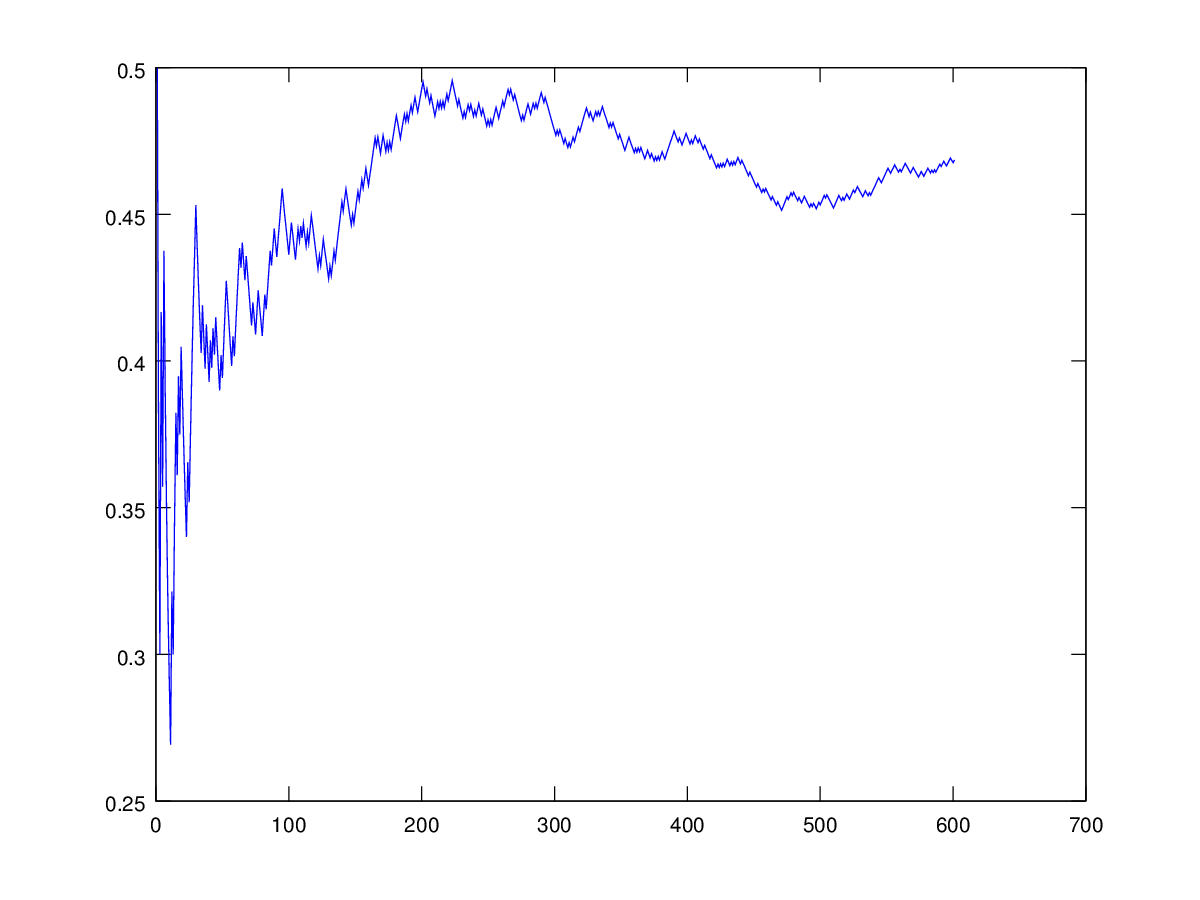
\includegraphics[width=0.7\textwidth]{polya1.png}
\caption{Simulaci\'on de urna de Polya}
\label{Urna de Polya}
\end{figure}
\end{proof}

\item Vuelva a correr el c\'odigo varias veces y escriba sus impresiones sobre lo que est\'a sucediendo.
\end{enumerate}
\end{ejercicio}

\begin{problema}[Ejercicios sueltos sobre martingalas]
\mbox{}\begin{enumerate}
\item Sea $\paren{X_n,n\geq 0}$ una sucesi\'on $\paren{\F_n}$-adaptada. Pruebe que\begin{esn}
\sum_{k=1}^n X_k-\espc{X_k}{\F_{k-1}}, \quad n\geq 0
\end{esn}es una $\paren{\F_n}$-martingala.
\begin{proof}
A�adiremos la suposici\'on de que $\paren{X_n,n\geq 0} \in L_1$. Definamos
\[M_n:=\sum_{k=1}^n X_k-\espc{X_k}{\F_{k-1}},\]
de manera que $M_0=0$ y 
\[M_n= M_{n-1} + X_n - \mean (X_n |\F_{n-1})\tres\forall n\in\entpos .\]
$M_0$ es $\F_0$-medible y es un elemento de $L_1$. Se demostrar\'a lo mismo para $M_n$ con $n\in\entpos$ por inducci\'on. As\'i que, asumamos que $M_{n}$ es $\F_{n}$-medible y es un elemento de $L_1$. Entonces
\[M_{n+1}=M_n + X_n - \mean (X_n |\F_{n-1}),\]
donde $\mean (X_n |\F_{n-1})$ es $\F_{n-1}$-medible y por lo tanto es $\F_{n}$-medible. Por hip\'otesis, $M_n$ es $\F_{n}$-medible, y lo mismo sucede con $X_n$. La suma de funciones $\F_{n}$-medibles es $\F_{n}$-medible y en consecuencia, $M_{n+1}$ es $\F_{n}$-medible. Tambi\'en, 
\begin{align*}
\mean (|M_{n+1}|)& \le \mean (|M_n|) + \mean (|X_n|) + \mean (|\mean (X_n |\F_{n-1})|)\\
& \le \mean (|M_n|) + \mean (|X_n|) + \mean (\mean (|X_n| |\F_{n-1}))\\
& \le \mean (|M_n|) + \mean (|X_n|) + \mean (|X_n|) < \infty,
\end{align*}
por lo tanto, $M_{n+1}\in L_1$, terminando con la inducci\'on.

Ahora,
\begin{align*}
\mean (M_{n+1}|\F_n ) & = \mean (M_{n} + X_{n+1} - \mean (X_{n+1} |\F_{n}) | \F_n)\\
& = \mean (M_{n} | \F_n) + \mean (X_{n+1} | \F_n) - \mean (\mean (X_{n+1} |\F_{n}) | \F_n)\\
& = M_{n} + \mean (X_{n+1} | \F_n) - \mean (X_{n+1} |\F_{n})\\
& \nota{(Por la $\F_n$-medibilidad de $M_{n}$ y $\mean (X_{n+1} | \F_n)$)}\\
& = M_n,
\end{align*}
y en consecuencia, $M$ es una $\F_n$-martingala.
\end{proof}
\item{Descomposici\'on de Doob para submartingalas}: Sea \(X=\paren{X_n}_{n\in\na}\) una submartingala. Pruebe que \(X\) se puede descomponer de manera \'unica como \(X=M+A\) donde \(M\) es una martingala y \(A\) es un proceso previsible con \(A_0=0\). Sugerencia: Asuma que ya tiene la descomposici\'on y calcule esperanza condicional de \(X_{n+1}\) dada \(X_n\). 
\begin{proof}
Como $X$ es una submartingala, entonces es $\F_n$ adaptado y est\'a en $L_1$. Por lo tanto, podemos aplicar el inciso anterior, es decir, hacer
\[N_n:=\sum_{k=1}^n X_k-\espc{X_k}{\F_{k-1}}\]
o equivalentemente, $N_0=0$ y 
\[N_n= N_{n-1} + X_n - \mean (X_n |\F_{n-1})\tres\forall n\in\entpos ,\]
que ser\'a una $\F_n$-martingala. Si definimos $M_n:=N_n + X_0$ para todo $n\in\nats$, entonces $M_n$ sigue siendo $\F_n$-medible ($X_0$ es $\F_n$-medible para todo $n\in\nats$), est\'a en $L_1$ y
\[\mean (M_{n+1} | \F_n ) = \mean (N_{n+1} + X_0| \F_n) = N_n + X_0 = M_n,\]
por lo tanto, $M_n$ tambi\'en es $\F_n$-martingala.

Si definimos un proceso $A$ tal que
\begin{align*}
A_n & := - M_n + X_n\\
& = -\left(\sum_{k=1}^n X_k-\espc{X_k}{\F_{k-1}} + X_0\right) + X_n\\
& = \sum_{k=1}^n \espc{X_k}{\F_{k-1}}- X_k + X_n - X_0\\
& = \sum_{k=1}^{n} \espc{X_k}{\F_{k-1}}- X_{k-1}\\
\end{align*}

Para demostrar que $A$ es previsible, notemos que todos los t\'erminos $\espc{X_k}{\F_{k-1}}$ y $X_{k-1}$ son $\F_{k-1}$-medibles (m\'as generalmente, ser\'an $\F_{n-1}$-medibles, ya que $\F_{k-1}\subset\F_{n-1}n$), la suma de ellos sigue siendo $\F_{n-1}$-medible y por lo tanto, $A_n$ es $\F_{n-1}$-medible.

Equivalentemente, podemos decir que $A_0=0$ y
\[A_n= A_{n-1} + \espc{X_n}{\F_{n-1}}- X_{n-1}.\]
Para demostrar que esta sucesi\'on de $A_n$ es no-decreciente, veamos que para todo $n\in\entpos$,
\begin{align*}
A_n-A_{n-1} & = \espc{X_n}{\F_{n-1}}- X_{n-1}
&\ge X_{n-1} - X_{n-1}\\
& \nota{(Por que $X$ es sub-martingala)}\\
&=0,
\end{align*}
es decir, sus incrementos son no negativos (c.s.), y por lo tanto, $A$ ser\'a no decreciente.

De la definici\'on inicial de $A$, es f\'acil notar que $X_n=M_n + A_n$ para todo $n\in\nats$.

Para demostrar la unicidad de esta representaci\'on, supongamos que existen otros procesos $M'$ y $A'$ que cumplen las mismas caracter\'isticas y $X_n=M_n' + A_n'$ para todo $n\in\nats$. Entonces, para cualquier $n\in\nats$,
\[M_n' + A_n' = M_n + A_n\]
\[\ent (M_n'-M_{n+1}') + (A_n'-A_{n+1}') = (M_n-M_{n+1}) + (A_n-A_{n+1}) \]
\[\ent \mean ( (M_n'-M_{n+1}') + (A_n'-A_{n+1}')|\F_n) = \mean ((M_n-M_{n+1}) + (A_n-A_{n+1})|\F_n) \]
y usando la propiedad de martingala de $M$ y $M'$ y la previsibilidad de $A$, 
\[\ent A_n'-A_{n+1}' = A_n -A_{n+1},\]
es decir, los incrementos en $A'$ y $A$ son los mismos, y como $A_0'=A_0=0$, entonces $A_n'=A_n$ para todo $n\in\nats$. Adem\'as,
\[M_n'=X_n-A_n'=X_n-A_n=M_n\tres\forall n\in\nats,\]
demostrando la unicidad (casi segura) de esta descomposici\'on.
\end{proof}
\item Sea \(S_n=\xi_1+\cdots+\xi_n\) donde las variables \(\xi\) son independientes y \(\xi_i\) tiene media cero y varianza finita \(\sigma_i^2\). Pruebe que si \(\sum_i \sigma_i^2<\infty\) entonces \(S_n\) converge casi seguramente y en \(L_2\) conforme \(n\to\infty\). Construya un ejemplo de variables aleatorias \(\xi_i\) tales que la serie \(\sum_i \xi_i\) sea casi seguramente absolutamente divergente y casi seguramente condicionalmente convergente (considere ejemplos simples!). Explique heur\'isticamente por qu\'e cree que suceda esto.
%Ser\'a que \sum_i\abs{x_i}=\infty casi seguramente si \sum_i\abs\esp{\xi_i}=\infty? 
\begin{proof}
Consideraremos $\F_n=\sigma (\xi_1,\dots ,\xi_n)$. Notemos que $\mean (\xi_i)=0$ para todo $i\in\nats$, de manera que $S_n$ es una caminata aleatoria centrada en cero, con $\xi_i\in L_1$, y por lo demostrado en clase, ser\'a una $\F_n$-martingala. Tambien notemos que $Var (\xi_i) = \mean ((\xi_i - \mean (\xi_i))^2) = \mean (\xi_i^2)$, es decir, la varianza es exactamente igual al segundo momento. Lo mismo es cierto para $X_n$ (ya que de nuevo, es una caminata aleatoria centrada en cero y $\mean (X_n)=0$ para todo $n\in\nats$). Entonces,
\begin{align*}
\mean (S_n^2) & = Var (S_n) = Var (\xi_1+\cdots+\xi_n)\\
&= \sum_{i=1}^n Var (\xi_i) \nota{(Por independencia de las $\xi_i$'s)}\\
&\le \sum_{i=1}^\infty Var (\xi_i).
\end{align*}
Lo anterior es v\'alido para toda $n\in\nats$, de manera que 
\[\sup_n S_n \le \sum_{i=1}^\infty Var (\xi_i) < \infty.\]
Aplicando el Teorema de convergencia de martingalas acotadas en $L_p$ con $p=2$, entonces $S_n$ converge c.s. y en $L_2$ a un $S_\infty\in\L_2$.

Para un ejemplo, considerese v.a.i. $\xi_i$ que toman los valores $-1/i$ \'o $1/i$, cada una con probabilidad $1/2$. Es claro que $\mean (\xi_i) = 0$ y
$Var (\xi_i ) = \mean (\xi_i^2) = (-1/i)^2\cdot 0.5 + (1/i)^2\cdot 0.5 = 1/i^2$.
Despu\'es,
\begin{align*}
\sum_{i=1}^\infty Var (\xi_i ) = \sum_{i=1}^\infty \frac{1}{i^2}<\infty , 
\end{align*}
y en consecuencia de la demostraci\'on anterior, $S_n$ converge c.s. y en $L_2$ a un elemento $S_\infty\in L_2$.

Para ver que la serie no es absolutamente convergente, basta ver que $|\xi_i | = 1/i$, de manera que
\[\sum_{i=1}^\infty \mean (|\xi_i |) = \sum_{i=1}^\infty \frac{1}{i}=\infty ,\]
por lo tanto, diverge.
\end{proof}
\item Sean \(X\) y \(Y\) dos martingalas (respecto de la misma filtraci\'on) y tales que \(\esp{X_i},\esp{Y_i}<\infty\) para toda \(i\). Pruebe la siguiente f\'ormula de integraci\'on por partes: $$ \esp{X_nY_n}-\esp{X_0Y_0}=\sum_{i=1}^n \esp{\paren{X_i-X_{i-1}}\paren{Y_i-Y_{i-1}}} . $$
\begin{proof}
Se necesitara que $Y_i, X_i \in L_2$ , y de esta manera, $\mean (X_i Y_j) < \infty$ para todo $i,j\in\nats$ (por desigualdad de Cauchy-Schwarz) y el problema est\'a bien definido. La demostraci\'on se har\'a por inducci\'on.

As\'i pues, cuando $n=0$, ambos lados de la igualdad ser\'an igual a $0$, por lo que \'esta se cumple.
Ahora, supngamos que la igualdad es v\'alida para $n$. Entonces
\begin{align*}
\sum_{i=1}^{n+1} & \esp{\paren{X_i-X_{i-1}}\paren{Y_i-Y_{i-1}}}\\ 
& = \sum_{i=1}^{n} \esp{\paren{X_i-X_{i-1}}\paren{Y_i-Y_{i-1}}} + \esp{\paren{X_{n+1}-X_{n}}\paren{Y_{n+1}-Y_{n}}}\\
& =\esp{X_nY_n}-\esp{X_0Y_0} + \esp{\paren{X_{n+1}-X_{n}}\paren{Y_{n+1}-Y_{n}}}\\
& = \esp{X_nY_n}-\esp{X_0Y_0} + \left(\mean (X_{n+1}Y_{n+1}) - \mean (X_{n}Y_{n+1}) - \mean (X_{n+1}Y_{n}) + \mean (X_{n}Y_{n})\right)\\
& = 2\esp{X_nY_n}-\esp{X_0Y_0} + \mean (X_{n+1}Y_{n+1}) - \mean (\mean (X_{n}Y_{n+1}|\F_n)) - \mean (\mean (X_{n+1}Y_{n}|\F_n))\\
& = 2\esp{X_nY_n}-\esp{X_0Y_0} + \mean (X_{n+1}Y_{n+1}) - \mean (X_{n}\mean (Y_{n+1}|\F_n)) - \mean (Y_{n}\mean (X_{n+1}|\F_n))\\
& \nota{(Por $\F_n$-medibilidad de $X_n$ y $Y_n$)}\\
& = 2\esp{X_nY_n}-\esp{X_0Y_0} + \mean (X_{n+1}Y_{n+1}) - \mean (X_{n}Y_n) - \mean (Y_{n}X_n)\\
& \nota{(Por que $Y$ y $X$ son martingalas)}\\
& = 2\esp{X_nY_n}-\esp{X_0Y_0} + \mean (X_{n+1}Y_{n+1}) - 2\mean (X_{n}Y_n)\\
& = \esp{X_{n+1}Y_{n+1}}-\esp{X_0Y_0},
\end{align*}
terminando con la inducci\'on y la demostraci\'on.
\end{proof}
\item{Desigualdad de Azema-Hoeffding, tomado de \cite[E14.2, p.237]{MR1155402}}
        \begin{enumerate}
        \item Muestre que si \(Y\) es una variable aleatoria con valores en \([-c,c]\) y media cero entonces, para \(\theta\in\re\)
                        $$\esp{e^{\theta Y}}\leq\imf{\cosh}{\theta c}\leq \imf{\exp}{\frac{1}{2}\theta^2c^2}. $$
\begin{proof}
Definamos la funci\'on $f(y)=e^{y \theta}$. $f(\cdot )$ es una funci\'on convexa. Adem\'as notemos que las siguientes igualdades se cumplen 
\begin{align*}
\frac{(c+Y)}{2c} + \frac{(c-Y)}{2c} = 1,
\end{align*}
donde cada sumando es $\le 1$ debido a que $|Y|\le c$ (esto nos servir\'a mas adelante al usar la convexidad de $f$). Tambi\'en notemos que se cumple la igualdad
\[\theta Y = (c \theta) \frac{(c+Y)}{2c} + (-c \theta ) \frac{(c-Y)}{2c},\]
y as\'i pues, tendremos que
\begin{align*}
\exp {(\theta Y)} & = \exp \left((c \theta) \frac{(c+Y)}{2c} + (-c \theta ) \frac{(c-Y)}{2c}\right)\\
& \le \frac{(c+Y)}{2c}\exp (c \theta) + \frac{(c-Y)}{2c}\exp (-c \theta )\\
& \nota{(Usando la definici\'on de convexidad sobre los puntos $f(c)$ y $f(-c)$).}
\end{align*}
Sacando esperanza y usando que $\mean (Y) = 0$, tenemos que
\[\mean (\exp {(\theta Y)}) \le \frac{c}{2c}\exp (c \theta) + \frac{c}{2c}\exp (-c \theta ) = \frac{e^{c\theta}+e^{-c\theta}}{2}= \cosh (\theta c).\]

La segunda desigualdad notemos que desarrollando cada serie de Taylor de $e^{x} + e^{-x}$, los t\'erminos impares de las series se anular\'an mientras que los pares coincidir\'an y se sumar\'an 2 veces. Cuando dividimos entre 2 para obtener la funci\'on $\cosh (x)$, al final quedara la suma de los t\'erminos pares (hablando acerca de la serie de Taylor de $e^x$). Es decir,
\[\cosh (x) = \sum_{n=0}^\infty \frac{x^{2n}}{(2n)!}\le\sum_{n=0}^\infty \frac{x^{2n}}{2^n(n!)}=\sum_{n=0}^\infty \frac{(x^2 /2)^n}{n!} = e^{x^2 /2},\]
donde se us\'o la desigualdad $2n! \le 2^n (n!)$, que es f\'acil de notar debido a que $2n!$ es toda la multiplicaci\'on de los n\'umeros $1$ hasta $2n$, mientras que $2^n (n!)$ corresponde a la multiplicaci\'on de solamente los n\'umeros pares anteriores (e iguales a) $2n$.
\end{proof}
        \item Pruebe que si \(M\) es una martingala nula en cero tal que para algunas constantes \(\paren{c_n,n\in\na}\) se tiene que
                        $$\abs{M_n-M_{n-1}}\leq c_n\quad\forall n $$
                        entonces, para \(x>0\)
                        $$
                        \proba{\max_{k\leq n} M_k\geq x}\leq \imf{\exp}{\frac{x^2}{2\sum_{k=1}^n c_k^2}}.
                        $$
\begin{proof}
Si $M$ es una martingala, entonces si le aplicamos la funci\'on convexa $f(M_n)=e\theta M_n$, este nuevo proceso ser\'a sub-martingala no negativa (por clase. Supongamos que $\theta > 0$ (de hecho, despu\'es se elegir\'a un valor conveniente para $\theta$), entonces la funci\'on $f$ es invertible y entonces los eventos $\{\max_{k\le n} M_x> x\}$ es equivalente a $\{\max_{k\le n} e^{\theta M_k}> e^{\theta x}\}$. Usando la Desigualdad m\'aximal de Doob para este \'ultimo evento, tenemos que que 
\[\p (\max_{k\le n} M_x> x) = \p (\max_{k\le n} e^{\theta M_k}> e^{\theta x})\le e^{-\theta x}\mean (e^{\theta M_n}).\]
Veamos que
\begin{align*}
\mean (e^{\theta M_n}) & = \mean (\mean (e^{\theta M_n}|\F_{n-1}))\\
& = \mean (\mean (e^{\theta M_{n-1}}e^{\theta (M_n - M_{n-1})}|\F_{n-1}))\\
& = \mean ( e^{\theta M_{n-1}} \mean (e^{\theta (M_n - M_{n-1})}|\F_{n-1}))\\
& \le \mean ( e^{\theta M_{n-1}}\cosh (\theta c_n))\nota{(*)}\\
& = \cosh (\theta c_n)\mean ( e^{\theta M_{n-1}})\\
& \le \exp (\theta^2 c_n^2 / 2),
\end{align*}
donde (*) es v\'alido por que en la demostraci\'on del inciso anterior pudimos haber sacado esperanza condicional en lugar de esperanza y en lugar de usar la propiedad $\mean (Y)=0$, usar\'iamos la propiedad $\mean (Y|\F) = 0$. Pero justamente, como en este caso tenemos que por ser martingala, $\mean ( M_n - M_{n-1}|\F_{n-1}) = 0$, de manera que la desigualdad se sigue cumpliendo.

Si repetimos este procedimiento $n$ pasos, llegar\'iamos a que 
\[\mean (e^{\theta S_n})\le \prod_{i=1}^n \exp (\theta^2 c_i^2/2)= \exp \left( \left(\theta^2\sum_{i=1}^n c_i^2\right) /2\right). \]
Entonces,
\[\p (\max_{k\le n} M_x> x) \le e^{-\theta x}\mean (e^{\theta M_n}) = \exp \left( -\theta x + \left(\theta^2 \sum_{i=1}^n c_i^2\right) /2\right).\]

Recordemos que esto es v\'alido para toda $\theta > 0$. De esta manera, si $x>0$, podemos tomar a 
\[\theta:= \frac{x}{\sum_{i=1}^n c_i},\]
y as\'i, 
\[-\theta x + \frac{\theta^2 \sum_{i=1}^n c_i^2}{2} = \frac{-x^2}{\sum_{i=1}^n c_i} + \frac{x^2}{2\sum_{i=1}^n c_i} = \frac{-x^2}{2\sum_{i=1}^n c_i},\]
y en resumen,
\[\p (\max_{k\le n} M_x> x) \le \exp \left(\frac{-x^2}{2\sum_{i=1}^n c_i}\right)\]
\end{proof}
        \end{enumerate}
\end{enumerate}
\end{problema}
\begin{problema}
Sea $S_n=\sum_{i=1}^n X_i$ donde $X_1,X_2,\ldots$ son iid. Sea\begin{esn}
\imf{\phi}{\lambda}=\esp{e^{\lambda S_n}}\in (0,\infty].
\end{esn}
\begin{enumerate}
\item Pruebe que si existen $\lambda_1<0<\lambda_2$ tales que $\imf{\phi}{\lambda_i}<\infty$ entonces $\imf{\phi}{\lambda}<\infty$ para toda $\lambda\in [\lambda_1,\lambda_2]$. Sugerencia: escriba $\lambda=a\lambda_1+(1-a)\lambda_2$ para alg\'un $a\in [0,1]$ y aplique la desigualdad de H\"older. A partir de ahora se asume la premisa de este inciso.
\begin{proof}
Sea $\lambda\in [\lambda_1 , \lambda_2 ]$ con representaci\'on $\lambda = a\lambda_1 + (1-a)\lambda_2$ p.a. $a\in [0,1]$. Entonces, usando la desigualdad de Holder con $p=1/a$ y $q=1/(1-a)$,
\begin{align*}
\phi (\lambda ) & = \mean (e^{\lambda S_n})= \mean (e^{a\lambda_1 S_n + (1-a)\lambda_2 S_n})=\mean (e^{a\lambda_1 S_n} e^{(1-a)\lambda_2 S_n})\\
& \le \mean(e^{\lambda_1 S_n})^{a}\mean(e^{\lambda_2 S_n})^{1-a} = \phi (\lambda_1 )^a \phi (\lambda_2)^{1-a}<\infty ,
\end{align*} 
domostrando la finitud de $\phi (\lambda )$ para cualquier $\lambda\in [\lambda_1 , \lambda_2 ]$.
\end{proof}
\item Pruebe que $\esp{\abs{S_n}^k}<\infty$ para toda $k\geq 0$. 
\begin{proof}
Sea $\lambda_0\in (0,\min (-\lambda_1 ,\lambda_2 ))$. Notemos que \[(0,\min (-\lambda_1 ,\lambda_2 ))\subset [\lambda_1,\lambda_2]\] y 
\[(-\min (-\lambda_1 ,\lambda_2 ),0)\subset [\lambda_1,\lambda_2],\] entonces por el inciso anterior, $\phi (\lambda_0 )<\infty$ y $\phi (-\lambda_0 )<\infty$. Consideremos la expansi\'on de Taylor de la funci\'on $\exp (\cdot )$ evaluada en $|\lambda_0 S_n|$, es decir
\[e^{|\lambda_0 S_n|}=\sum_{i=0}^\infty \frac{|\lambda_0 S_n |^i}{i!}\ge \frac{\lambda_0^k|S_n |^k}{k!} \]
de manera que
\[|S_n |^k\le \frac{e^{|\lambda_0 S_n|} k!}{\lambda_0^k}\le \frac{(e^{\lambda_0 S_n} + e^{-\lambda_0 S_n})k!}{\lambda_0^k},\]
y tomando esperanzas
\[\mean ( |S_n |^k) \le \frac{(\mean (e^{\lambda_0 S_n}) + \mean (e^{-\lambda_0 S_n}))k!}{\lambda_0^k}= \frac{(\phi (\lambda_0 ) + \phi (-\lambda_0 ))k!}{\lambda_0^k}<\infty ,\]
finalizando la demostraci\'on.
\end{proof}
\item Sea $M^\lambda_t=e^{\lambda S_t}/\imf{\phi}{\lambda}$. Argumente que si $M^n$ es el proceso dado por\begin{esn}
M^n_t=\left.\frac{\partial^n}{\partial \lambda^n}\right|_{\lambda=0}M^\lambda_t,
\end{esn}entonces $M^n$ es una martingala para toda $n$. 
\begin{proof}
Debemos demostrar la integrabilidad, medibilidad y propiedad de martingala para cada $n\in\nats$. Por ahora, asumamos que $M^n$ es integrable para toda $n$ (ese problema lo dejaremos para el final). 
Definamos
\[\tilde M^n_t = \frac{\partial^n}{\partial \lambda^n}M^\lambda_t\]
En clase se demostr\'o que el caso $\tilde M^0$ era martingala. Siguiendo los pasos de una inducci\'on, supongamos que el caso $\tilde M^n$ tambi\'en es una martingala. Si por ahora suponemos que el operador derivada puede salir de la esperanza condicional, tendremos entonces que para todo $s<t$,
\begin{align*}
\mean\left(\tilde M_t^{n+1}|\F_s\right) & = \mean\left(\frac{\partial^{n+1}}{\partial \lambda^{n+1}}M^\lambda_t|\F_s\right)\\
& = \frac{\partial}{\partial \lambda} \left(\mean\left(\frac{\partial^n}{\partial \lambda^n}M^\lambda_t |\F_s\right)\right)\\
& = \frac{\partial}{\partial \lambda} \left(\tilde M^n_s\right)\nota{(Por hip. de inducci\'on)}\\
& = \frac{\partial}{\partial \lambda}\tilde M^n_s = \tilde M^{n+1}_s,
\end{align*}
lo cual tambien ser\'a cierto para el proceso $M^n = \tilde M^n|_{\lambda=0}$.

A continuaci\'on se dar\'a una explicaci\'on de porque es posible intercambiar el operador derivada con la esperanza condicional que dar\'a tambi\'en como resultado auxiliar, la medibilidad de las derivadas de orden $n$. La derivada (por la derecha) de una funci\'on $f$ medible derivable, est\'a definida por
\[\frac{\partial}{\partial \lambda}f(\lambda) = \lim_{n\to \infty} \frac{f(\lambda +1/n)-f(\lambda )}{1/n}.\]
(En nuestro caso, la funci\'on ser\'a $M_t^\lambda$, que es integrable y est\'a correctamente definida para una vecindad de del $0$, por lo que si nos tomamos $\lambda\in (\lambda_1,\lambda_2)$, podemos tomar en lugar de de la sucesi\'on $\lambda + 1/n$, alguna subsucesi\'on que est\'e contenida en $(\lambda_1,\lambda_2)$ y as\'i no tendremos problemas con integrabilidad). 
Notemos que esta derivada es un limite de funciones medibles, por lo tanto, \'esta ser\'a tambi\'en medible (de aqu\'i es donde se demuestra la medibilidad de cada $M^n$). Si la derivada de $f$ es integrable, podemos aplicar el teorema de convergencia dominada para esperanza condicional para intercambiar la esperanza condicional con el l\'imite, aplicar definici\'on de derivada de nuevo y tendr\'iamos como conclusi\'on que podemos cambiar el operador derivada con la esperanza condicional.

Por lo tanto, bastar\'a con demostrar que cada 
\[\frac{\partial^n}{\partial \lambda^n}M^\lambda_t\]
es integrable para toda $n$.
Para ello, enunciemos la expansi\'on de Taylor  respecto a $\lambda$ de $M^\lambda_t$ alrededor de $a$, donde $a\in (\lambda_1,\lambda_2)$,
\[M^\lambda_t = \sum_{n=0}^\infty \frac{(\lambda-a)^n}{n!}\left.\frac{\partial^n}{\partial \lambda^n}\right|_{\lambda=a}M^\lambda_t\ge 0.\]
Si aplicamos esperanza, la anterior igualdad ser\'a v\'alida para todo $\lambda\in (\lambda_1,\lambda_2)\backslash\{a\}$ y m\'as a\'un, utilizando el teorema de convergencia acotada para intercambiar suma con esperanza, tendremos que 
\[1 = \sum_{n=0}^\infty \frac{(\lambda-a)^n}{n!}\mean\left(\left.\frac{\partial^n}{\partial \lambda^n}\right|_{\lambda=a}M^\lambda_t\right).\]
Como se tiene que $\lambda\neq a$, esto implica que 
\[-\infty <\mean\left(\left.\frac{\partial^n}{\partial \lambda^n}\right|_{\lambda=a}M^\lambda_t\right)<\infty.\]
Para concluir correctamente, deber\'iamos demostrar una de 2 cosas que el valor absoluto de la funci\'on 
\[\left.\frac{\partial^n}{\partial \lambda^n}\right|_{\lambda=a}M^\lambda_t\]
 es integrable; sin embargo, no me fue posible deducirlo correctamente.
\end{proof}
\item Calcule las primeras $4$ martingalas resultantes si $\proba{X_i=\pm 1}=1/2$. Util\'icelas para calcular el valor de $\esp{T^2}$ donde\begin{esn}
T=\min\set{n\geq 0: S_n\in\set{-a,b}}\end{esn}
\begin{proof}
Usando los 3 incisos anteriores, mediante c\'alculos auxiliados por computadora (las derivadas se ponen feas en el tercer y cuarto paso), tenemos que
\begin{align*}
M^1_t & = S_t\\
M^2_t & = S_t^2 - t\\
M^3_t & = S_t^3 -3 t S_t\\
M^4_t & = S_t^4 - 6 t S_t^2 + 3 t^2 + 2t.
\end{align*}
Es justamente $M^4_t$ la martingala que nos interesa utilizar como medio para calcular $\mean (T^2)$. El resultado visto en clase del Problema de la Ruina, nos dice que $\prob(S_T=-a)=b/(a+b)$, $\prob(S_T=-b)=a/(a+b)$ y que $\mean (T)=ab$.
Por lo tanto,
\begin{align*}
\mean (S_T) & =0\\
\mean (S_T^2) & =ab\\
\mean (S_T^3) & =ab(a-b)\\
\mean (S_T^4) & =(ab(a^3+b^3))/(a+b).
\end{align*}

Aplicando el Teorema de Muestreo Opcional de Doob para la cuarta martingala, tendremos que
\[\mean (S_T^4-6TS_T^2+3T^2+2T)=0\]
Por lo que
\begin{align*}
\esp{T^2} & \frac{\mean (-S_T^4 +6TS_T^2-2T)}{3}\\
& =\frac{-(ab(a^3+b^3))/(a+b) + 6\mean (TS_T^2) -2ab}{3}.
\end{align*}

Se resolvi\'o el problema en el caso $a=b$, de manera que tendremos que $\mean(TS_T^2)=a^2 \mean(T) = a^4$, y la f\'ormula se reduce a
\[\mean(T^2)=\frac{5a^4-2a^2}{3}.\]
No fue posible calcular $\mean(TS_T^2)$ en general.
\end{proof}
\end{enumerate}

\defin{Categor\'ias:} Caminatas aleatorias, muestreo opcional, ejemplos de martingalas. 
\end{problema}

\begin{problema}
Sea $M$ una $\paren{\F_n}$-martingala. Pruebe que si $T$ es un tiempo de paro finito entonces $\esp{M_T}=\esp{M_0}$ bajo cada una de las siguientes condiciones:
\begin{enumerate}
\item $M$ es acotada.
\begin{proof}
$T\wedge n$ es un tiempo de paro acotado, as\'i que usando Teorema de Muestreo Opcional, tenemos que $\mean (M_{T\wedge n}) = \mean (M_0)$. Adem\'as, como $T$ es finito, entonces $M_{T\wedge n}\rightarrow M_T$ c.s. cuando $n\rightarrow\infty$, hecho que se utilizar\'a en las siguientes demostraciones.
Si $M$ es acotada, entonces existe un $a\in\reals$ tal que $M_n < a$ para todo $n\in\nats$. Entonces la sucesi\'on $M_{T\wedge n} < a$ para todo $n\in\nats$. As\'i pues, usando TCA,
\[\mean (M_T) = \mean (\lim_{n\rightarrow\infty} M_{T\wedge n}) = \lim_{n\rightarrow\infty} \mean (M_{T\wedge n}) = \mean (M_0).\]
\end{proof}
\item $T$ es integrable y la sucesi\'on $\paren{M_n-M_{n-1}}$ es acotada.
\begin{proof}
Sea $c\in\reals$ tal que $|M_i-M_{i-1}|<c$ para toda $i\in\entpos$, lo cual es posible por que las diferencias son acotadas. De nuevo, como $T\wedge n$ es un tiempo de paro, por Teorema del Muestreo Opcional, se tiene que $\mean(M_{T\wedge n}-M_0) = 0$. Entonces
\[|M_{T\wedge n}-M_0| = |\sum_{i=1}^{T\wedge n} (M_i-M_{i-1})|\le\sum_{i=1}^{T\wedge n} |(M_i-M_{i-1})|\le\sum_{i=1}^{T\wedge n}c=c\cdot T\wedge n \le c\cdot T.\]
Pero $\mean(c \cdot T) = c\cdot\mean (T) <\infty$, de manera que tenemos una cota para $|M_{T\wedge n}-M_0|$ que es integrable. Aplicando TCD,
\[\mean(M_{T}-M_0)=\lim_{n\rightarrow\infty}\mean(M_{T\wedge n}-M_0)=0.\]
\end{proof}
\item $\paren{M_{n\wedge T}}$ es uniformemente integrable. 
\begin{proof}
Se usar\'a que $T\wedge n$ es un tiempo de paro finito y que por Teorema de Muestreo Opcional, $\mean (M_{T\wedge n}) = \mean (M_0)$.
Por que $T$ es un tiempo de paro finito, entonces $M_{T\wedge n}\rightarrow M_T$ c.s. cuando $n\rightarrow \infty$. Como tenemos que $\paren{M_{n\wedge T}}$ es uniformemente integrable, esto implica que $M_{T\wedge n}\rightarrow M_T$ en $L_1$ cuando $n\rightarrow \infty$. Esto implica que $\mean (M_T)=\lim_{n\rightarrow\infty} \mean (M_{T\wedge n}) = \mean (M_0)$.
\end{proof}
\end{enumerate}

\defin{Categor\'ias: } Muestreo opcional. 
\end{problema}

\begin{problema}
Sea $M$ una $\paren{\F_n}$-martingala con saltos acotados. Sean\begin{esn}
C=\set{\limsup M_n=\liminf M_n\in\re}\quad\text{y}\quad D=\set{\limsup M_n=-\infty\text{ y }\limsup M_n=\infty}.
\end{esn}Pruebe que $\proba{C\cup D}=1$. Deduzca que las caminatas aleatorias centradas con saltos acotados oscilan. Sugerencia: Para cada $K>0$ defina\begin{esn}
T=\min\set{n\geq 0: \abs{M_n}\geq K}
\end{esn}y aplique el teorema de convergencia de martingalas a $M^T$. 

Sea $M$ una caminata aleatoria no trivial con saltos integrables en $-1,0,1,\ldots$ y  media cero. Pruebe que $\proba{M\text{ converge en }\na}=0$ y  concluya que $\liminf M_n=-\infty$ casi seguramente. (Este resultado permitir\'a dar una prueba adicional de que un Galton-Watson cr\'itico se extingue).  Sugerencia: proceda como en el p\'arrafo anterior y pruebe la integrabilidad uniforme de $M_{T\wedge n},n\in\na$.
\begin{proof}
Sea $T_a$ el tiempo de paro correspondiente a la primera vez que el proceso $M_n$ cruza por debajo del nivel $-a$ o por arriba el nivel $a$, es decir,
\[T_a = \inf \{t\ge 0: M_t \le -a \mbox{ \'o } M_t \ge a\}.\]
Notemos que el evento $\{T_a=n\}$ depende solamente de los primeros $n$ pasos del proceso $M_n$, por lo tanto efectivamente es un tiempo de paro. Si se tienen saltos acotados, digamos por $C$, entonces se tiene que $|M_{T_a\wedge n}| < a + C$, y as\'i $\sup_{n\in\nats} \mean (|M_{T_a\wedge n}|)\le a + C<\infty$. Si se tienen saltos integrables, digamos $X_i$, entonces $|M_{T_a\wedge n}| \le a + |X_{T_a\wedge n}|$ y 
\begin{align*}
\lim_{t\to\infty}& \sup_{n\in\nats}\mean (|M_{T_a\wedge n}|\mathds{1}_{|M_{T_a\wedge n}|>t}) \le \lim_{t\to\infty}\sup_{n\in\nats}\mean ((a + |X_{T_a\wedge n}|)\mathds{1}_{|X_{T_a\wedge n}|>t-a})\\
& = \lim_{t\to\infty}a\prob (|X_{1}|>t-a) +\mean ( |X_{1}|\mathds{1}_{|X_{1}|>t-a})\nota{(Por que las $X_i$ son i.i.d.)}\\
& = 0\nota{(Por la integrabilidad de los saltos),}
\end{align*}
es decir, $M_{T_a\wedge n}$ es uniformemente integrable. En consecuencia, para cualquiera de los 2 casos (saltos acotados o integrables), se tendr\'a que $M_{T_a\wedge n}$ converge c.s. a una v.a. en $L_1$.

Ahora, estudiaremos el proceso $M_n$ bajo los \'unicos 2 eventos posibles; \[\set{\liminf M_n > -\infty \mbox{ \'o } \limsup M_n < \infty}\] y \[\set{\limsup M_n=-\infty\text{ y }\limsup M_n=\infty}\] (de hecho, \'este \'ultimo corresponde a al evento $D$). Para el primero, notemos que bajo el evento $\set{T_a=\infty}$, $M_{T_a\wedge n} = M_n$ y como $M_{T_a\wedge n}$ converge, $M_n$ tambi\'en lo har\'a. 
Esto es cierto para cualquier $a\in\nats$ y entonces $M_n$ tambi\'en converger\'a sobre el evento
 \[\set{\liminf M_n > -\infty \mbox{ \'o } \limsup M_n < \infty} = \cup_{a\in\nats}\set{T_a = \infty}.\]
Notemos que la convergencia de $M_n$ a un elemento de $L_1$ implica que $M_n$ no puede converger a $\infty$ \'o $-\infty$. En conclusi\'on se tendr\'a que el evento $\set{\liminf M_n > -\infty \mbox{ \'o } \limsup M_n < \infty}$ es igual al evento $C$ definido inicialmente. Como esos son l\'as \'unicas 2 posibilidades, se tendr\'a que $\prob (C\cup D)=1.$

Falta demostrar que cualquier caminata aleatoria (no trivial) centrada debe de oscilar. Se ha demostrado en clase que una caminata de este tipo es una martingala. Como es no trivial, existe un $l\neq 0$ tal que $\prob (X_i=l) = \epsilon >0$. Entonces 
\[\sum_{i=1}^\infty \prob (X_i=l) = \infty,\]
y por BC, el evento  $\set{X_i=l}$ suceder\'a i.o. con probabilidad $1$, de manera que es imposible que la caminata se estabilice en alg\'un nivel. Por lo tanto se tendr\'a que $\prob (C) = 0$ y por lo tanto la caminata oscila.

Nota: la discusi\'on anterior es v\'alida para cualquier tipo de caminata centrada no trivial, ya sea con saltos acotados o integrables.
\end{proof}

\defin{Categor\'ias: } Teoremas de convergencia de martingalas
\end{problema}

\begin{problema}
Sean $X_1,X_2,\ldots$ variables aleatorias intercambiables:\begin{esn}
\paren{X_1,\ldots, X_n}\stackrel{d}{=}\paren{X_{\pi_1},\ldots, X_{\pi_n}}
\end{esn}para cada permutaci\'on $\sigma$ de $\set{1,\ldots,n}$. 
\begin{enumerate}
\item Para $\G,\h$ sub$\sigma$-\'algebras de $\F$ definimos a $\G\vee\h=\sag{\G\cup\h}$. Sea \begin{esn}
\G^n=\sag{\imf{f}{X_1,\ldots, X_n}: \fun{f}{\re^n}{\re}\text{ es sim\'etrica}}\vee\sag{X_{n+1},X_{n+2},\ldots}. 
\end{esn}Pruebe que $\G^n,n\geq 1$ es una filtraci\'on al rev\'es. Sea $\G$ su intersecci\'on.
\begin{proof}
Se har\'a una demostraci\'on parcial de este hecho, ya que no conozco la manera correcta de generar a la familia de funciones medibles y simetricas. Analizando los incisos posteriores y el uso que se le da a $\G^n$, es preferible definir la $\sigma$-\'algebra
\[\G^n=\sag{\imf{f}{X_1,\ldots, X_n}: f(x_1,\dots x_n)=\sum_{\beta\in\Theta_n} f_1(x_{\beta_1})\cdots f_n(x_{\beta_n})}\vee\sag{X_{n+1},X_{n+2},\ldots},\]
donde $\Theta_n$ es el conjunto de todas las permutaciones de los primeros $n$ elementos y cada $f_i$ es una funci\'on real medible. Claramente la funci\'on $f$ definida de esa manera es sim\'etrica; el problema es que al parecer no se generan a todas las funciones sim\'etricas mediante esta construcci\'on, por ejemplo, no se puede generar a la funci\'on $\max (x_1,\dots ,x_n)$; sin embargo, cubre una buena parte de las funciones con las que usualmente trabajamos.

Bajo esta nueva definici\'on, basta con demostrar que los elementos que generan a $\G_{n+1}$ tambi\'en se encuentran en $\G_n$. El conjunto $\sag{X_{n+2},X_{n+2},\ldots}$ obviamente se encuentra en $\sag{X_{n+1},X_{n+2},\ldots}\subset \G_n$. Entonces, para cada sucesi\'on de funciones medibles $\{f_i(\cdot)\}$, tomemos su funci\'on sim\'etrica de las primeras $n+1$ v.a., de manera que
\begin{align*}
\sum_{\beta\in\Theta_{n+1}} & f_1(X_{\beta_1})\cdots f_{n+1}(X_{\beta_{n+1}})\\
& = \sum_{\beta\in\Theta_{n+1}} f_{\beta_1}(X_1) \cdots f_{\beta_{n+1}}(X_{n+1})\\
& = \sum_{i=1}^{n+1}\left(\sum_{\beta\in\Theta_{n}^{i}} f_{\beta_1}(X_1)\cdots f_{\beta_{n}}(X_{n})f_{i}(X_{n+1})\right)\\
& \tres \nota{(Donde $\Theta_n^i$ son las permutaciones de $1$ a $n+1$ excluyendo $i$)}\\
& = \sum_{i=1}^{n+1}\{f_{i}(X_{n+1}) \sum_{\beta\in\Theta_{n}^{i}} f_{\beta_1}(X_1)\cdots f_{\beta_{n}}(X_{n}),
\end{align*}
de donde notamos que esta funci\'on se puede expresar como una funci\'on sim\'etrica de las primeros $n$ v.a. por una funci\'on medible de la v.a. $X_{n+1}$ y por lo tanto, tambien es $\G_n$ medible. De esta manera, acabamos de demostrar que $\G_{n+1}\subset \G_n$ y entonces $G$ es una filtraci\'on al rev\'es.
\end{proof}
\item Para cada $A\in\mc{B}_{\re}$, defina a\begin{esn}
\imf{\Xi_n}{A}=\frac{1}{n}\sum_{i=1}^n \indi{X_i\in A}.
\end{esn}Pruebe que\begin{esn}
\probac{X_1\in A}{\G^n}=\imf{\Xi_n}{A}. 
\end{esn}?`Por qu\'e puede definir a  $\imf{\Xi}{A}=\lim_{n\to\infty}\imf{\Xi_n}{A}$?
\begin{proof}
Claramente la funci\'on $\Xi_n (A)$ es una funci\'on sim\'etrica, dado que permutar el orden de los sumandos no cambia el total. Esto implica que $\Xi_n (A)$ es $\G^n$-medible y
\[\Xi_n (A) = \mean (\Xi_n (A)|\G^n) = \frac{1}{n}\sum_{i=1}^n \mean (\mathds{1}_{X_i\in A}|\G^n).\]
Para demostrar que $\mean (\mathds{1}_{X_i\in A}|\G^n) = \mean (\mathds{1}_{X_1\in A}|\G^n)$ para todo $i\in\nats$, tendremos que demostrar que para cualquier funci\'on sim\'etrica $g:\mathds{R}^n\to\mathds{R}$,
\[\mean (g(X_1,X_2,\dots , X_n)\mathds{1}_{X_i\in A})=\mean (g(X_1,X_2,\dots , X_n)\mathds{1}_{X_1\in A}).\]
As\'i pues, sea $\beta(\cdot )$ una permutaci\'on que manda la entrada $i$ a $1$. La intercambiabilidad en distribuci\'on de $X_1 , X_2 , \dots , X_n$ implica que 
\begin{align*}
\mean (g(X_1,X_2,\dots , X_n)\mathds{1}_{X_i\in A}) & = \mean (g(X_{\beta (1)},X_{\beta (2)},\dots , X_{\beta (n)})\mathds{1}_{X_{\beta(i)}\in A})\\
& = \mean (g(X_{\beta (1)},X_{\beta (2)},\dots , X_{\beta (n)})\mathds{1}_{X_{1}\in A})\\
& = \mean (g(X_1,X_2,\dots , X_n)\mathds{1}_{X_i\in A})\nota{(Por que $g$ es sim\'etrica),}
\end{align*}
de manera que $\mean (\mathds{1}_{X_i\in A}|\G^n) = \mean (\mathds{1}_{X_1\in A}|\G^n)$ y en consecuencia $\p ({X_i\in A}|\G^n) = \p ({X_1\in A}|\G^n)$, concluyendo que 
\[\Xi_n (A) = \frac{1}{n}\sum_{i=1}^n \mean (\mathds{1}_{X_i\in A}|\G^n) = \p ({X_1\in A}|\G^n).\]

Entonces se tendr\'a que $\Xi_n(A) = \mean (\mathds{1}_{X_1\in A}|\G^n)$, donde $\mathds{1}_{X_1\in A}\in\L_1$ y $\G^n$ es una filtraci\'on al rev\'es, entonces, por el Teorema de Levy Hacia Abajo, existir\'a un limite cuando $n\to\infty$, y de hecho, el l\'imite, al cual llamaremos $\Xi (A)$, ser\'a $\mean (\mathds{1}_{X_1\in A}|\cap_{n\in\nats}\G^n) = \mean (\mathds{1}_{X_1\in A}|\G) = \p ({X_1\in A}|\G)$.

Nota:Este resultado bien pudo ser obtenido para demostrar la igualdad a $\p ({X_l\in A}|\G)$ para cualquier $l\in\nats$.
\end{proof}
\item Al considerar a la martingala\begin{esn}
\frac{1}{n\paren{n-1}}\sum_{1\leq i<j\leq n}\indi{X_i\in A}\indi{X_j\in A},
\end{esn}pruebe que $\probac{X_1\in A,X_2\in A}{\G}=\probac{X_1\in A}{\G}\probac{X_2\in A}{\G}$. Extienda la afirmaci\'on de independencia condicional anterior a $X_1,\ldots, X_n$. 
\begin{proof}
El primer paso, ser\'a demostrar que para todo $i\neq j$,
\[\mean (\mathds{1}_{X_i\in A}\mathds{1}_{X_j\in A}|\G^n) = \mean (\mathds{1}_{X_1\in A}\mathds{1}_{X_2\in A}|\G^n).\] 
Es decir, tendremos que demostrar que para cualquier funci\'on sim\'etrica $g:\mathds{R}^n\to\mathds{R}$,
\[\mean (g(X_1,X_2,\dots , X_n)\mathds{1}_{X_i\in A}\mathds{1}_{X_j\in A})=\mean (g(X_1,X_2,\dots , X_n)\mathds{1}_{X_1\in A}\mathds{1}_{X_2\in A}).\]
As\'i pues, sea $\beta(\cdot )$ una permutaci\'on que manda la entrada $i$ a $1$ y $j$ a $2$. La intercambiabilidad en distribuci\'on de $X_1 , X_2 , \dots , X_n$ implica que 
\begin{align*}
\mean & (g(X_1,X_2,\dots , X_n)\mathds{1}_{X_i\in A}\mathds{1}_{X_j\in A})  = \mean (g(X_{\beta (1)},X_{\beta (2)},\dots , X_{\beta (n)})\mathds{1}_{X_{\beta(i)}\in A}\mathds{1}_{X_{\beta(j)}\in A})\\
& = \mean (g(X_{\beta (1)},X_{\beta (2)},\dots , X_{\beta (n)})\mathds{1}_{X_{1}\in A}\mathds{2}_{X_{1}\in A})\\
& = \mean (g(X_1,X_2,\dots , X_n)\mathds{1}_{X_i\in A}\mathds{1}_{X_{2}\in A})\nota{(Por que $g$ es sim\'etrica),}
\end{align*}
de manera que $\mean (\mathds{1}_{X_i\in A}\mathds{1}_{X_j\in A}|\G^n) = \mean (\mathds{1}_{X_1\in A}\mathds{2}_{X_i\in A}|\G^n)$ y en consecuencia $\p ({X_i\in A, X_j\in A}|\G^n) = \p ({X_1\in A, X_2\in A}|\G^n)$, concluyendo que 
\[\frac{1}{n(n-1)}\sum_{0<i\neq j\le n} \mean (\mathds{1}_{X_i\in A}\mathds{1}_{X_j\in A}|\G^n) = \p ({X_1\in A},{X_2\in A}|\G^n),\]
ya que existir\'an $n(n-1)$ sumandos id\'enticos.

Notemos que $\mean (\mathds{1}_{X_1\in A}\mathds{1}_{X_2\in A}|\G^n)$ es una martingala reversa (respecto a $n$), donde $\mathds{1}_{X_1\in A}\mathds{1}_{X_2\in A}\in\L_1$ y $\G^n$ es una filtraci\'on al rev\'es, entonces, por el Teorema de Levy Hacia Abajo, existir\'a un limite cuando $n\to\infty$ que ser\'a 
\[\mean (\mathds{1}_{X_1\in A}\mathds{1}_{X_2\in A}|\cap_{n\in\nats}\G^n) = \mean (\mathds{1}_{X_1\in A}\mathds{1}_{X_2\in A}|\G) = \p (X_1\in A, X_2 \in A|\G).\] En conclusi\'on, se demostr\'o que efectivamente la suma propuesta es una martingala y esta tiene como limite a $\p (X_1\in A, X_2 \in A|\G)$. La demostraci\'on de estas propiedades para el caso general $X_1,X_2,\cdots ,X_k$ es totalmente an\'aloga.

Ahora, 
\begin{align*}
\frac{\sum_{i=1}^n \mathds{1}_{X_i \in A}}{n}\frac{\sum_{j=1}^n \mathds{1}_{X_j \in A}}{n} & = \frac{\sum_{0<i\neq j\le n} \mathds{1}_{X_i \in A}\mathds{1}_{X_j \in A}}{n^2} + \frac{\sum_{i=1}^n \mathds{1}_{X_i \in A}^2}{n^2}\\
& = \frac{n-1}{n}\frac{\sum_{0<i\neq j\le n} \mathds{1}_{X_i \in A}\mathds{1}_{X_j \in A}}{n(n-1)} + \frac{\sum_{i=1}^n \mathds{1}_{X_i \in A}}{n^2}.
\end{align*}
Notemos que todos los l\'imites cuando $n\to \infty$ existen (por el inciso anterior y por lo demostrado inicialmente) , y de hecho la \'ultima sumatoria est\'a acotada por $n$, de manera que al ser dividida por $n^2$, en el l\'imite la \'ultima fracci\'on ser\'a igual a $0$. Es decir, se tendr\'a que
\[\lim_{n\to\infty}\frac{\sum_{i=1}^n \mathds{1}_{X_i \in A}}{n}\frac{\sum_{j=1}^n \mathds{1}_{X_j \in A}}{n} = \lim_{n\to\infty}\frac{n-1}{n}\frac{\sum_{0<i\neq j\le n} \mathds{1}_{X_i \in A}\mathds{1}_{X_j \in A}}{n(n-1)}\]
\[\ent\left(\lim_{n\to\infty}\frac{\sum_{i=1}^n \mathds{1}_{X_i \in A}}{n}\right)\left(\lim_{n\to\infty}\frac{\sum_{j=1}^n \mathds{1}_{X_j \in A}}{n}\right) = \lim_{n\to\infty}\frac{\sum_{0<i\neq j\le n} \mathds{1}_{X_i \in A}\mathds{1}_{X_j \in A}}{n(n-1)}\]
\[\ent \p (X_1\in A|\G)\p (X_2\in A|\G) = \p (X_1\in A, X_2 \in A|\G).\]
Para demostrar el caso general, se har\'a por inducci\'on, es decir, se supondr\'a que la formula es v\'alida para $k-1$ y por lo tanto bastar\'a demostrar que 
\[\probac{X_1\in A,X_2\in A,\dots ,X_k\in A}{\G}=\probac{X_1\in A,\dots, X_{k-1}}{\G}\probac{X_k\in A}{\G}.\]
Entonces
\begin{align*}
& \frac{\sum_{i_1\neq\dots\neq i_{k-1}} \mathds{1}_{X_{i_1} \in A,\dots ,X_{i_{k-1}} \in A}}{n(n-1)\cdots (n-k+2)}\frac{\sum_{j=1}^n \mathds{1}_{X_j \in A}}{n} \\
& = \frac{\sum_{i_1\neq\dots\neq i_{k-1}\neq i_k} \mathds{1}_{X_{i_1} \in A,\dots ,X_{i_{k-1}}\in A ,X_{i_k}\in A}}{n\cdot n(n-1)\cdots (n-k+2)} \\
&\tres + \frac{\sum_{i_1\neq\dots\neq i_{k-1} \wedge i_k=i_l} \mathds{1}_{X_{i_1} \in A,\dots ,X_{i_{k-1}}\in A ,X_{i_k}\in A}}{n\cdot n(n-1)\cdots (n-k+2)}\\
& = \frac{n-k+1}{n}\frac{\sum_{i_1\neq\dots\neq i_{k-1}\neq i_k} \mathds{1}_{X_{i_1} \in A,\dots ,X_{i_{k-1}}\in A ,X_{i_k}\in A}}{n(n-1)\cdots (n-k+2)(n-k+1)} \\
&\tres + \frac{\sum_{i_1\neq\dots\neq i_{k-1}} \mathds{1}_{X_{i_1} \in A,\dots ,X_{i_{k-1}}\in A}}{n\cdot n(n-1)\cdots (n-k+2)}\\
&\tres\nota{(Por que como $i_k=i_l$, existe un evento que esta repetido).}
\end{align*}
La \'ultima sumatoria tiene $n(n-1)\cdots (n-k+2)$ elementos, por lo tanto estar\'a acotada por ese n\'umero, de manera que dividiendo entre $n\cdot n(n-1)\cdots (n-k+2)$ y haciendo $n\to\infty$, esta \'ultima fracci\'on ser\'a $0$. Los dem\'as limites existen y en conclusi\'on tendremos que 
\[\probac{X_1\in A,\dots, X_{k-1}}{\G}\probac{X_k\in A}{\G}=\probac{X_1\in A,X_2\in A,\dots ,X_k\in A}{\G},\]
finalizando la demostraci\'on.
\end{proof}
\end{enumerate}

\defin{Cagegor\'ias: }Teorema de convergencia de martingalas, teorema de de Finetti.
\end{problema}

\begin{ejercicio}
\mbox{}
\begin{enumerate}
\item Ejecute y explique la funci\'on del siguiente c\'odigo en Octave. Comente qu\'e teoremas del curso (y del curso de probabilidad) son importantes para interpretar la figura.
\begin{proof}
El programa realiza $10000$ trayectorias del experimento de as urnas de Polya y localiza los resultados. Cada una de estas trayectorias se compone de sacar y meter bolas $1000$ veces en total. En clase se demostr\'o que cuando hacemos tender al infinito el n\'umero de veces que sacamos y metemos bolas, la proporci\'on de bolas tend\'ia a una v.a. con distribuci\'on Beta. Y esto es justamente lo que sucede en el programa; se compara la distribuci\'on emp\'irica de las $10000$ realizaciones con la distribuci\'on de una v.a. Beta.
\begin{figure}
\centering
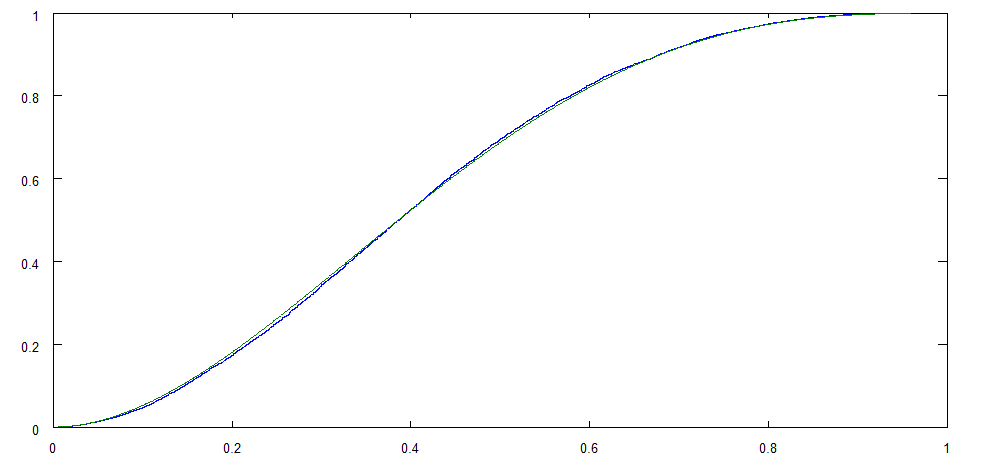
\includegraphics[width=0.7\textwidth]{1beta0.png}
\caption{Polya vs. Beta}
\label{Polya vs. Beta}
\end{figure}
\end{proof}


\item Ejecute y explique la funci\'on del siguiente c\'odigo en Octave. Incluya una gr\'afica en la que la longitud de la variable k sea mayor a 1000. (Puede modificar el programa...) En la gr\'afica observara un esbozo de la trayectoria de un proceso de ramificaci\'on continuo (en una escala distinta...).
\begin{proof}
Se trata de una poblaci\'on donde cada individuo tiene 0 o 2 hijo con probabilidad $1/2$ para cada opci\'on. Es decir, a media de la progenie es $1$; entonces este proceso de ramificaci\'on se arruinar\'a con probabilidad $1$. En la figura \ref{GW} se presenta una reaizaci\'on del c\'odigo propuesto.

\begin{figure}
\centering
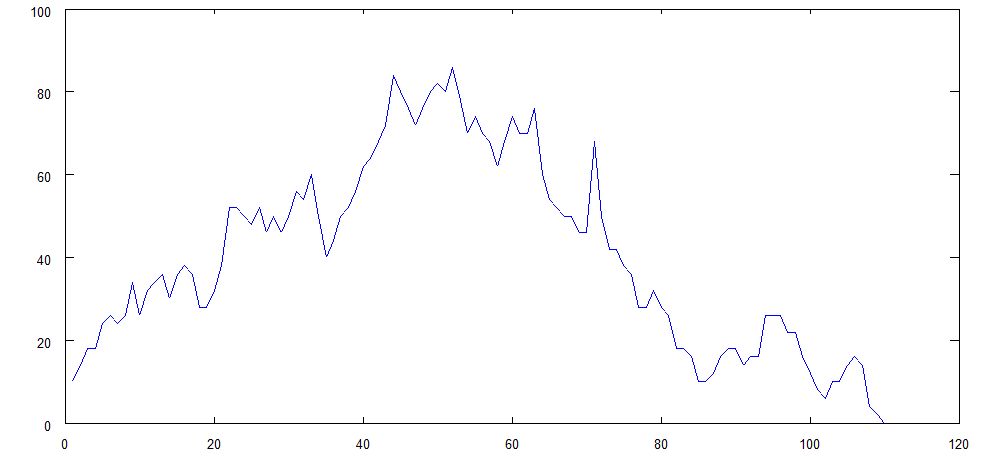
\includegraphics[width=0.7\textwidth]{2beta1.png}
\caption{GW}
\label{GW}
\end{figure}

A continuaci\'on se presenta el c\'odigo modificado que permite obtener una poblaci\'on que haya durado m\'as de 1000 generaciones.

\begin{lstlisting}
k=[10];
aux=k(length(k));
while (length(k)<1000)
k=[10];
aux=k(length(k));
while (aux>0 && length(k)<1100)
k=[k;2*binornd(aux,.5)];
aux=k(length(k));
endwhile
endwhile
plot(k)
\end{lstlisting}
y la Figura \ref{GW >1000} es una realizaci\'on del anterior c\'odigo.
\begin{figure}
\centering
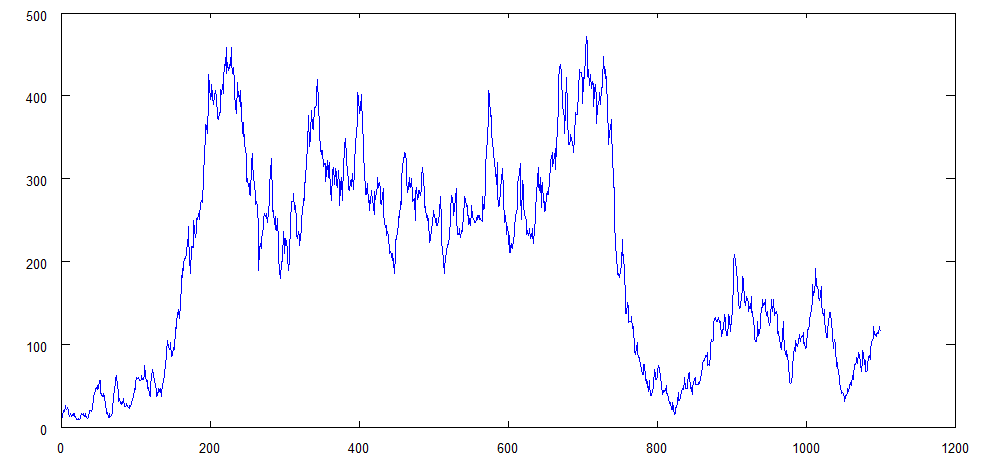
\includegraphics[width=0.7\textwidth]{3beta3.png}
\caption{GW $>1000$}
\label{GW >1000}
\end{figure}
\end{proof}
\end{enumerate}
\end{ejercicio}

%
%\begin{problema}
%Sean $\F_1,\F_2,\ldots $ y $\G$ sub\sa s de $\F$. Decimos que $\F_1,\F_2,\ldots$ son condicionalmente independientes dada $\G$ si para cualquier $H_i$ que sea $\F_i$ medible y acotada se tiene que\begin{esn}
%\espc{H_1\cdots H_n}{\G}=\espc{H_1}{\G}\cdots \espc{H_n}{\G}.
%\end{esn}
%\begin{enumerate}
%\item ?`Qu\'e quiere decir la independencia condicional cuando $\G=\set{\oo,\emptyset}$?
%\item Pruebe que $F_1$ y $\F_2$ son condicionalmente independientes dada $\G$ (denotado $\condind{\F_1}{\F_2}{\G}$) si y s\'olo si para cualquier $H$ que sea $\F_1$-medible y acotada se tiene que\begin{esn}
%\espc{H}{\F_2,\G}=\espc{H}{\G}.
%\end{esn}
%\item Pruebe que $\F_1,\F_2,\ldots, $ son condicionalmente independientes dada $\G$ si y s\'olo si para cada $n\geq 1$, $\F_{n+1}$ es condicionalmente independiente de $\F_1,\ldots, \F_n$ dada $\G$. 
%\end{enumerate}
%
%\defin{Categor\'ias: } Esperanza condicional, Independencia condicional.
%\end{problema}
%
%\begin{problema}
%Sea $\mu$ una distribuci\'on de progenie y defina $\tilde \mu_j=\mu_{j+1}$. Sea $S=\paren{S_n}$ una caminata aleatoria con distribuci\'on de salto $\tilde\mu$. Sea $k$ un entero no-negativo y defina recursivamente\begin{esn}
%Z_0=k=C_0,\quad Z_{n+1}=k+S_{C_n}\quad\text{y} C_{n+1}=C_n+Z_{n+1}.
%\end{esn}
%\begin{enumerate}
%\item Pruebe que $Z_n\geq 0$ para toda $n$ y que si $Z_n=0$ entonces $Z_{n+1}=0$.
%\item Pruebe que $C_n$ es un tiempo de paro para la filtraci\'on can\'onica asociada a $S$.
%\item Pruebe que $Z$ es un proceso de Galton-Watson con ley de progenie $\mu$. 
%\item Pruebe que si $S$ alcanza $-1$ entonces existe $n$ tal que $Z_n=0$. Deduzca que si la media de $\mu$ es $1$ entonces $Z$ se extingue. (Sugerencia: utilice un ejercicio anterior sobre martingalas con saltos acotados hacia abajo.) 
%\end{enumerate}
%
%\defin{Categor\'ias: } Caminatas aleatorias, Procesos de Galton-Watson%, Propiedad de Markov fuerte.
%\end{problema}
%
%\begin{problema}
%Sea $\mu$ una distribuci\'on de progenie y defina $\tilde \mu_j=\mu_{j+1}$. Sea $\nu$ una distribuci\'on en $\na$. Consideremos a dos caminatas aleatorias $S=\paren{S_n}$  y $T$ con  distribuci\'ones de salto $\tilde\mu$ y $\nu$.
%\begin{enumerate}
%\item ?`Qu\'e significa que $S$ y $T$ sean independientes? As\'umalo.
%\item Sea $k$ un entero no-negativo y defina recursivamente\begin{esn}
%Z_0=k=C_0,\quad Z_{n+1}=k+S_{C_n}+T_n\quad\text{y} C_{n+1}=C_n+Z_{n+1}.
%\end{esn}
%\item Pruebe que $Z_n\geq 0$ para toda $n$.
%\item Pruebe que $C_n=k\in\F^S_k\cap\F^T_n$.
%\item Pruebe que $Z$ es un proceso de Galton-Watson con inmigraci\'on.
%\end{enumerate}
%
%\defin{Categor\'ias: } Caminatas aleatorias, Procesos de Galton-Watson, Construcci\'on de procesos estoc\'asticos
%\end{problema}
%
%\begin{problema} %Construcci\'on tipo Poisson 
%Sean $\mu$ y $\nu$ una distribuci\'on de progenie y de inmigraci\'on. Sean $Y_1,Y_2,\ldots$ independientes y de ley $\nu$. Suponga que condicionalmente a $Y$, $X^0,X^1,X^2,\ldots$ son procesos de Galton-Watson independientes tales que $X^0_0=k$ y $X^k_0=Y_k$ para $k\geq 1$. Pruebe que si\begin{esn}
%Z_n=\sum_{k=0}^n X^k_{n-k},
%\end{esn}entonces $Z$ es un proceso de Galton-Watson con distribuciones de progenie e inmigraci\'on $\mu$ y $\nu$ que comienza en $k$. 
%
%\defin{Categor\'ias: } Procesos de ramificaci\'on
%\end{problema}
%
%\begin{problema}
%Para cada par de medidas de probabilidad en $\na^\na$ $\p_1$ y $\p_2$ definimos a la convoluci\'on de $\p_1$ y $\p_2$, denotada $\p_1 *\p_2$, como la distribuci\'on de $\paren{S^1_k+S^2_k,k\geq 0}$ donde $S^1$ y $S^2$ son independientes y de distribuciones $\p_1$ y $\p_2$ respectivamente.
%\begin{enumerate}
%\item ?` Cu\'al es la relaci\'on entre las distribuciones finito-dimensionales de $\p_1$, $\p_2$ y $\p_1*\p_2$?
%\item Sea $\p_k^\mu$ la distribuci\'on de un proceso de Galton-Watson  de ley de reproducci\'on $\mu$ que comienza en $k$. Pruebe que $\p_{k_1}*\p_{k_2}=\p_{k_1+k_2}$.
%%\item Caracterizaci\'on de leyes markovianas con la propiedad de ramificaci\'on.
%\end{enumerate}
%
%\defin{Categor\'ias: } Distribuciones finito-dimensionales, Procesos de ramificaci\'on.
%\end{problema}
\end{document}